% Modelo de TCC do Bacharelado em Ciência da Computação da UNIFESP 
% Baseado no Modelo de Documentos Academicos do ABNTex2  

\documentclass[	12pt, Times, openright, twoside, a4paper, english, brazil]{abntex2}

% ---
% Pacotes fundamentais 
% ---
\usepackage{cmap}				% Mapear caracteres especiais no PDF
%\usepackage{lmodern}			% Usa a fonte Latin Modern			
\usepackage{times}
\usepackage[T1]{fontenc}			% Selecao de codigos de fonte.
\usepackage[utf8]{inputenc}		% Codificacao do documento (conversão automática dos acentos)
\usepackage{lastpage}			% Usado pela Ficha catalográfica
%\usepackage{natbib}
\usepackage{indentfirst}			% Indenta o primeiro parágrafo de cada seção.
\usepackage{color}				% Controle das cores
\usepackage{graphicx}			% Inclusão de gráficos
\usepackage{enumerate}
\usepackage{enumitem}
% ---

% ---
% Pacotes de citações
% ---
\usepackage[brazilian,hyperpageref]{backref}	 % Paginas com as citações na bibl
\usepackage[alf]{abntex2cite}	% Citações padrão ABNT

% --- 
% CONFIGURAÇÕES DE PACOTES
% --- 

% ---
% Configurações do pacote backref
% Usado sem a opção hyperpageref de backref
\renewcommand{\backrefpagesname}{Citado na(s) página(s):~}
% Texto padrão antes do número das páginas
\renewcommand{\backref}{}
% Define os textos da citação
\renewcommand*{\backrefalt}[4]{
	\ifcase #1 %
		Nenhuma citação no texto.%
	\or
		Citado na página #2.%
	\else
		Citado #1 vezes nas páginas #2.%
	\fi}%
% ---

% numeração de figuras e tabelas 
\counterwithout{figure}{section}
\counterwithout{table}{section}

%\renewcommand\tablename{Tabela{\arabic{chapter}.}}

\newcommand{\bkc}[1]{{\color{blue}{#1}}} % revisão
\newcommand{\bko}[1]{{\color{red}{#1}}} % observação

% ---
% Informações de dados para CAPA e FOLHA DE ROSTO
% ---
\titulo{Estudo Comparado de Uniformes Operacionais para a Radiopatrulha}
\autor{Al Of PM Christian Ferreira da Silva\\Al Of PM Fernando Bandeira Soares}
\local{São Paulo, SP}
\data{Setembro de 2020}
\orientador{Maj PM Celso Ricardo de Souza}
\instituicao{%
  Polícia Militar do Estado de São Paulo
  \par
  Academia de Polícia Militar do Barro Branco
  \par
  Bacharelado em Ciências Policiais de Segurança e Ordem Pública}
\tipotrabalho{Trabalho de Graduação}
% O preambulo deve conter o tipo do trabalho, o objetivo, 
% o nome da instituição e a área de concentração 
\preambulo{Trabalho de conclusão de curso apresentado à Academia de Polícia Militar do Barro Branco - APMBB, como parte das atividades para obtenção do título de Bacharel em Ciências Policiais de Segurança e Ordem Pública.}
% ---

% informações do PDF
\makeatletter
\hypersetup{
     	%pagebackref=true,
		pdftitle={\@title}, 
		pdfauthor={\@author},
    	pdfsubject={\imprimirpreambulo},
	    pdfcreator={LaTeX with abnTeX2},
		pdfkeywords={abnt}{latex}{abntex}{abntex2}{trabalho acadêmico}, 
		colorlinks=true,       		% false: boxed links; true: colored links
    	linkcolor=blue,          	% color of internal links
    	citecolor=blue,        		% color of links to bibliography
    	filecolor=magenta,      		% color of file links
		urlcolor=blue,
		bookmarksdepth=4
}

\makeatother
% --- 
% --- 
% Espaçamentos entre linhas e parágrafos 
% --- 
% O tamanho do parágrafo é dado por:
\setlength{\parindent}{1.3cm}
% Controle do espaçamento entre um parágrafo e outro:
\setlength{\parskip}{0.2cm}  % tente também \onelineskip
% ---

% compila o indice
% ---
\makeindex
% ---

% ----
% Início do documento
% ----
\begin{document}
% Retira espaço extra obsoleto entre as frases.
\frenchspacing 

% ----------------------------------------------------------
% ELEMENTOS PRÉ-TEXTUAIS
% ----------------------------------------------------------
% \pretextual

% ---
% Capa
% ---
\begin{capa}
  \begin{center}
    {\ABNTEXchapterfont\bfseries\Large\MakeUppercase\imprimirinstituicao}
    \vspace*{\fill}\vspace*{\fill}
    
    
\includegraphics[width=.25\textwidth]{logo-apmbb.png}
    \vspace*{\fill}
    
    {\ABNTEXchapterfont\large\imprimirautor}
    \vspace*{\fill}
    
    {\ABNTEXchapterfont\bfseries\Large\MakeUppercase\imprimirtitulo}
    \vspace*{\fill}\vspace*{\fill}
    
   \imprimirlocal
   \end{center}
\end{capa}

% ---
% Folha de rosto
% (o * indica que haverá a ficha bibliográfica)
% ---
\imprimirfolhaderosto*
% ---

% ---
% Inserir folha de aprovação
% ---
% Isto é um exemplo de Folha de aprovação, elemento obrigatório da NBR
% 14724/2011 (seção 4.2.1.3). Você pode utilizar este modelo até a aprovação
% do trabalho. Após isso, substitua todo o conteúdo deste arquivo por uma
% imagem da página assinada pela banca com o comando abaixo:
%
% \includepdf{folhadeaprovacao_final.pdf}
%
\begin{folhadeaprovacao}
  \begin{center}
    {\ABNTEXchapterfont\large\imprimirautor}

    \vspace*{\fill}\vspace*{\fill}
    {\ABNTEXchapterfont\bfseries\Large\imprimirtitulo}
    \vspace*{\fill}
    
    \hspace{.45\textwidth}
    \begin{minipage}{.5\textwidth}
        \imprimirpreambulo
    \end{minipage}%
    \vspace*{\fill}
   \end{center}
    
   Trabalho aprovado em \_\_\_ de junho de 2021:

   \assinatura{\textbf{\imprimirorientador} \\ Orientador} 
   \assinatura{\textbf{Professor} \\ Convidado 1}
   \assinatura{\textbf{Professor} \\ Convidado 2}
   \assinatura{\textbf{Professor} \\ Convidado 3}
   %\assinatura{\textbf{Professor} \\ Convidado 4}
      
   \begin{center}
    \vspace*{0.5cm}
    {\large\imprimirlocal}
    \par
    {\large\imprimirdata}
    \vspace*{1cm}
  \end{center}
  
\end{folhadeaprovacao}
% ---

% ---
% Dedicatória
% ---
\begin{dedicatoria}
   \vspace*{\fill}
   \centering
   \noindent
   \textit{ Este trabalho é dedicado às minhas noites mal dormidas.} \vspace*{\fill}
\end{dedicatoria}
% ---

% ---
% Agradecimentos
% ---
\begin{agradecimentos}
Agradeço a Deus por tudo quanto faz em minha vida. 
\\À minha família, por suportar minha ausência durante minhas longas horas de estudos. 
\\Agradeço a todos os meus amigos, pois fazem tudo que podem para me ajudar nessa jornada. 
\\Agradeço à minha esposa, Letícia, que acredita em meu potencial e sem a qual, nada disso faria sentido. 
\\Agradeço a meu orientador, Bruno Kimura, por todo o suporte que me concede, por sempre arrumar tempo para me orientar em meios a tantos afazeres e por nunca deixar de responder meus inúmeros e-mails.


\end{agradecimentos}
% ---

% ---
% Epígrafe
% ---
\begin{epigrafe}
    \vspace*{\fill}
	\begin{flushright}
		\textit{``No que diz respeito ao empenho, ao compromisso, ao esforço, à dedicação, não existe meio termo. Ou você faz uma coisa bem feita ou não faz."\\(Airton Senna)}
	\end{flushright}
\end{epigrafe}
% ---

% ---
% RESUMOS
% ---

% resumo em português
\begin{resumo}

\par A Internet é uma ferramenta amplamente utilizada hoje em dia. Apesar de seu sucesso, a infraestrutura da Internet pouco mudou desde sua concepção até agora. No entanto, novas necessidades têm surgido e nem todas encontram soluções definitivas. A mobilidade de sistemas finais é uma dessas novas necessidades que surgiu com o aumento do uso de dispositivos móveis. 
\par É claro que esse problema tem sido tratado, mas com dificuldades e não da melhor forma. A dificuldade vem do nível de penetração que a Internet atingiu, tornando inviável que alterações em sua infraestrutura sejam feitas. Devido a isso, alguns serviços tratam a mobilidade na camada da aplicação, o que resulta no aumento da complexidade das aplicações e da pilha de protocolos nos sistemas finais.
\par Para contornar esse e outros problemas, tem-se buscado tornar a rede mais flexível. Com isso, surgiu um novo paradigma denominado Redes Definidas por Software (SDN). Através de SDN a rede torna-se programável, possibilitando que inovações sejam inseridas em sua infraestrutura, sem a necessidade de se alterar seus componentes.
\par Nesse trabalho será utilizado esse novo paradigma, na forma do protocolo Openflow, para estudar diferentes soluções de mobilidade dos sistemas finais na Internet. A construção de um ambiente de emulação e a obtenção de dados para avaliação dessas soluções são os principais objetivos desse trabalho de conclusão de curso.


 \vspace{\onelineskip}
    
 \noindent
 \textbf{Palavras-chaves}: SDN; OpenFlow; Ryu; Redes Móveis; Redes Modernas; Mobilidade.
\end{resumo}
%Tem uma pagina em branco aqui, mas não sei o porque...
% resumo em inglês
\begin{resumo}[Abstract]
 \begin{otherlanguage*}{english}

\par The Internet is a tool widely used nowadays. Despite its success, the Internet has had some small infrastructure changes over the years. However, new needs appeared, but definitive solutions have not been found to all of them. The end systems mobility is one of these new requirements that has appeared with the increasing usage of mobile devices.
\par Certainly, this problem has been treated, but not without difficulties not even in the best way. The obstacles come from the level of penetration that the Internet has reached, making it inviable for infrastructure changes to be made. Therefore, some services treat mobility at the application layer, resulting in the increasing application complexity and the processing overhead for the final system , which reduces device battery time.
\par The answer that has been sought is to make the network infrastructure more flexible, and with that, in the form of a new paradigm called Software Defined Network (SDN), that answer was found. Through SDN, it is possible to make the network programmable, enabling innovations to be inserted on the Internet, without changing its infrastructure.
\par This work use this new paradigm, in the form of Openflow protocol, to study different mobility solutions in the Internet. The construction of an emulation environment for these solutions and the obtainment of data for the evaluation of them, are the main objectives of this work piece.

   \vspace{\onelineskip}
 
   \noindent 
    \textbf{Palavras-chaves}: SDN; OpenFlow; Ryu; Mobile Networks; Modern Networks; Mobility.
 \end{otherlanguage*}
\end{resumo}

% ---
% inserir lista de ilustrações
% ---
\pdfbookmark[0]{\listfigurename}{lof}
\listoffigures*
\cleardoublepage
% ---

% ---
% inserir lista de tabelas
% ---
\pdfbookmark[0]{\listtablename}{lot}
\listoftables*
\cleardoublepage
% ---

% ---
% inserir lista de abreviaturas e siglas
% ---
\begin{siglas}
  \item[IETF] \textit{Internet Engineering Task Force}
  \item[IP] \textit{Internet Protocol}
  \item[ITU] \textit{International Telecommunications Union}
  \item[NAT] \textit{Network Address Translation}
  \item[OSI] \textit{Open System Interconnection}
  \item[QoS] \textit{Quality of Service}
  \item[RFC] \textit{Request For Comments}
  \item[SDN] \textit{Sofware-Defined Networks}
  \item[TCC] Trabalho de Conclusão de Curso
  \item[UML] \textit{User-Mode Linux}
  \item[UNIFESP] Universidade Federal de São Paulo
  \item[VM] \textit{Virtual Machine}
\end{siglas}
% ---

% ---
% inserir o sumario
% ---
\pdfbookmark[0]{\contentsname}{toc}
\tableofcontents*
\cleardoublepage
% ---

% ----------------------------------------------------------
% ELEMENTOS TEXTUAIS
% ----------------------------------------------------------
\textual

% ----------------------------------------------------------
% Introdução

% ----------------------------------------------------------
%Gostei desse texto, preciso melhorar o meu colando isso
\begin{comment} Tamanho sucesso, entretanto, traz consigo um problema para a comunidade de
pesquisa. Como grande parte da sociedade depende hoje da Internet em suas atividades
do dia-a-dia e tecnologias de acesso a rede se tornaram ` commodities de facil acesso, es- ´
tabilidade se tornou uma caracter´ıstica essencial da Internet. Isso significa que pesquisas
com novos protocolos e tecnologias nao s ˜ ao mais poss ˜ ´ıveis na Internet em geral, devido
ao risco de interrupc¸ao das atividades para as quais ela j ˜ a se tornou ferramenta essencial. ´
Nao s ˜ o isso, mas tamb ´ em a economia de escala poss ´ ´ıvel pelo crescimento da rede e a
larga adoc¸ao das tecnologias j ˜ a desenvolvidas inviabiliza a inserc¸ ´ ao de novas tecnologias ˜
que dependam de alterac¸oes do hardware a ser utilizado.
----------------------------------------------------------------------------------------------------
Dar uma olhada em DevoFlow ([Mogul et al. 2010)
----------------------------------------------------------------------------------------------------
\end{comment}

\chapter{Introdução}
\setcounter{page}{1}
%\par A Internet revolucionou o modo como as pessoas se relacionam, se comunicam e, resumidamente, na maneira como vivem. Inúmeras atividades, de um modo direto, ou indireto, utilizam a Internet como ferramenta para os mais diversos fins. Entre 2005 e 2015 o número de usuários conectados à rede mundial de computadores passou de 1 bilhão para 3,2 bilhões, segundo a União Internacional de Telecomunicações \cite{itu2016}, e nesses anos todos não houveram alterações significativas na infraestrutura da rede, apenas pequenas melhorias pontuais de modo a atender uma necessidade específica, como é o caso da utilização do mecanismo NAT \cite{rfc4787}, que permite um número de usuários maior do que números de IP disponíveis. Tais características demostram que a infraestrutura da Internet apresenta excelente escalabilidade e robustez, tendo sobrevivido ao grande aumento do número de usuários e carga das aplicações desde sua criação até o presente momento. No entanto, nesses anos todos, não foi só o número de usuários da Internet que mudou, novas necessidades têm surgido e nem todas encontram uma solução definitiva para atendê-las. Neste trabalho irá se estudar uma dessas novas necessidades: a mobilidade de um sistema final entre redes distintas. 

\par A Internet revolucionou o modo como as pessoas se relacionam, se comunicam e, em geral, na maneira como vivem. As mais diversas atividades do cotidiano, de um modo direto ou indireto, depende do acesso a serviços disponibilizados por servidores em redes remotas. De acordo com a União Internacional de Telecomunicações \cite{itu2016}, entre 2005 e 2015, o número de usuários conectados à rede mundial de computadores passou de 1 bilhão para 3,2 bilhões. A Internet tem acomodado o aumento exponencial de dispositivos e a carga de trabalho das aplicações através da operação de novos mecanismos na pilha de protocolos TCP/IP, os quais não foram inicialmente previstos em seu projeto de mais de 4 décadas. Um exemplo desses novos mecanismos é a tecnologia NAT \cite{rfc4787}, que permite um número de usuários maior do que números de IP disponíveis através da re-utilização de endereçamento privado. 

\par Nesse contexto, desde a sua existência, não houve alterações significativas na arquitetura da Internet. Observa-se adaptações pontuais em protocolos da pilha para atender necessidades específicas, conforme a demanda. Entretanto, ao longo desses anos todos, não foi só o número de usuários da Internet que mudou. Recentemente, aplicações têm demandado, cada vez mais, requisitos que não podem ser atendidos com a arquitetura ossificada da Internet. A mobilidade de um sistema final entre redes distintas é um requisito atual das aplicações que são executadas em dispositivos portáteis que ainda não possui solução nativa, a não ser pela adaptação de protocolos legados na pilha TCP/IP. Essa mobilidade é o objeto de estudo neste trabalho de conclusão de curso.


\section{Problema}
%\par Quando a Internet foi criada assumiu-se como verdade que cada sistema final era estático na rede e confiável, com a evolução das tecnologias e aumento do número de usuários da Internet, nenhum desses fatos permanecem.

%\par Segundo dados da Cisco, empresa conceituada e largamente conhecida do ramo redes, o tráfego de dados através de dispositivos móveis cresceu 63\% em 2016 e há previsão de que o número de dispositivos móveis conectados na Internet irá representar 20\% do total em 2021 \cite{CISCO2017}, são dispositivos tais como \textit{smartphones}, \textit{tablets}, os recém surgidos \textit{wearables} e ainda outros sistemas embarcados que estão em constante movimento entre redes. Dado as características da Internet, que em sua criação e evolução inicial, não previu esse tipo de comportamento, para que esses dispositivos permaneçam conectados de forma transparente para o usuário, diversas soluções foram surgindo. Inicialmente, e em muitos casos ainda, essa mobilidade é tratada na aplicação, ou seja, cada sistema final é encarregado de detectar a alteração de rede e tratar essa mudança de forma a impactar o menos possível para o usuário final, o que insere na rede um número muito grande de pacotes de controle e ainda torna maior a carga de processamento dos dispositivos, o que diminui, consideravelmente, a carga da bateria do dispositivo. Com o aumento dos dispositivos que possuem esse comportamento móvel, em relação a conexão com a Internet, viu-se que há uma necessidade de que a própria rede detecte, e trate, a mobilidade dos sistemas finais e assim começaram a surgir diferentes soluções para esse problema.

\par Quando a Internet foi criada, há mais de quatro décadas, assumiu-se a interconexão de poucos sistemas finais estáticos em uma rede confiável como demanda para a concepção do projeto. Com a evolução das tecnologias de transmissão e o aumento do número de usuários na Internet, nenhumas dessas premissas permaneceram.

\par Atualmente, cada vez mais é parte do cotidiano das pessoas o uso de dispositivos portáteis, tais como \textit{smartphones}, \textit{tablets}, e os recém surgidos \textit{wearables}, que são sistemas embarcados em movimento com os usuários. Segundo dados da Cisco~\cite{CISCO2017}, empresa conceituada e amplamente conhecida na indústria de telecomunicações, o tráfego de dados através de dispositivos móveis cresceu 63\% em 2016 e a previsão é que o número de dispositivos móveis conectados à Internet represente 20\% do total em 2021. Entretanto, o projeto da arquitetura da Internet, conforme em sua concepção, não considerou o ingresso de dispositivos portáteis na rede IP, e nem podia fazê-lo dado o cenário e a demanda inicial. Como na época os sistemas finais eram estáticos na rede, adotou-se um sistema de endereçamento estático que é utilizado tanto para identificação como para localização. As conexões entre os sistemas finais são então estabelecidas com base nesse endereço, quando esse é alterado, as conexões são interrompidas. Para que esses dispositivos permaneçam conectados de forma transparente enquanto o usuário se movimenta entre diferentes redes de acesso à Internet, diversas soluções e protocolos para tratar a mobilidade IP foram propostos na Literatura.

\par Dentre as diversas propostas existentes, a mobilidade é um problema tratável por soluções de diferentes camadas da pilha TCP/IP. Na camada de aplicação, o próprio processo de usuário (software) pode detectar a alteração de rede e tratar as rupturas de conexões e atrasos causados pela mobilidade de forma imperceptível para o usuário final. Exemplos dessas soluções são a arquitetura SMSL \cite{smsl} e os dois mecanismos apresentados em \cite{rockracks}. Na camada de transporte, protocolos legados, como TCP, são modificados para suportar mudança de endereçamento IP dos nós em mobilidade, como discutido em \cite{tcpmigrate} e \cite{snoeren}. Na camada de rede, adição de infraestrutura específica pode fazer com que o problema seja tratado pela rede e não mais pelos sistemas finais. Alguns dos trabalhos desenvolvidos com essa abordagem são \cite{avelar2013}, \cite{rfc3220} e \cite{rfc3775}. Dessa forma, não há consenso de camada ideal da pilha para tratar mobilidade. 

Embora soluções de transporte e aplicação sejam menos custosas (do ponto de vista de implantação e manutenção) e igualmente eficientes que soluções de camada de rede, todas essas são soluções que demandam adaptações ou modificações em protocolos legados na pilha TCP/IP. O estado de ``ossificação'' que a arquitetura da Internet atingiu é tal que impossibilita inovação na rede. Consequentemente, isso inviabiliza a implementação de soluções para os novos requisitos das aplicações (mobilidade, segurança, qualidade de experiência, etc) sem que haja modificações na pilha existente, causando, cada vez mais, complexidade e sobrecarga nos sistemas finais.

Nesse contexto, um novo paradigma de redes, denominado Redes Definidas por Software (SDN - \textit{Software-Defined Networks}) surgiu recentemente e tem atraído grande atenção da comunidade acadêmica e da indústria. Ao separar a operação do gerenciamento da rede em plano de dados (encaminhamento de pacotes) e plano de controle (decisões de encaminhamento), respectivamente, o paradigma SDN proporciona flexibilidade para implementação de solução de rede de forma independente da pilha existente. O controle da rede passa a ser centralizado logicamento num nó controlador, o qual dita regras de encaminhamento de pacotes para switches que possuem suporte ao protocolo OpenFlow, protocolo padrão SDN. Ao permitir que toda a rede seja programada no controlador, problemas de comunicação e requisitos variados das aplicações (como mobilidade dos seus dispositivos) podem ser resolvidos através de soluções algorítmicas, com suporte de técnicas de programação existentes, aprendizado de máquina, mineração e recuperação de informação, etc. Portanto, não há mais barreira que impeça a inovação na rede.

%o que insere na rede um número muito grande de pacotes de controle e ainda torna maior a carga de processamento dos dispositivos, o que diminui, consideravelmente, a carga da bateria do dispositivo
%BKC: isso não está coea quantidade de dados de controle para tratar mobilidade na aplicação é similar às soluções de protocolos de transporte e rede...

\section{Objetivos}
%\par O objetivo desse trabalho é analisar algumas das soluções propostas em artigos e pesquisas realizadas por diversos indivíduos ou grupos ao redor do mundo, pesquisas e artigos esses que abordaram a questão da mobilidade utilizando redes definidas por software, pois a utilização desse paradigma é uma tendência, dado o estado “ossificado” que a Internet atingiu e a flexibilidade que a utilização dessa abordagem proporciona. Quando se trabalha com Redes Definidas por Software, é possível obter um ambiente seguro para experimentação sem que fluxos normais de transmissão de dados sejam afetados. Irá ser utilizado o protocolo/padrão OpenFlow \cite{McKeown} na implementação dessas soluções pois esse é um padrão largamente aceito no mercado para redes definidas por software, sendo já disponibilizados diversos hardwares com suporte ao mesmo. Ao fim desse trabalho pretende-se apresentar dados que mostrem o desempenho dessas soluções e assim, poderá ser utilizado como fonte de dados para análises de viabilidade da implantação dessas soluções ou ainda para o desenvolvimento de uma nova solução. 

O objetivo principal deste trabalho é estudar as principais soluções de mobilidade propostas na Literatura que utilizam redes definidas por software. Pretende-se que esse estudo, além de teórico, no sentido de obter um levantamento do Estado da Arte, tenha um viés prático forte. Para tal, os objetivos específicos do trabalho são:
\begin{enumerate}
    \item Definir e implantar um ambiente experimental em emulador de rede que suporte o protocolo padrão OpenFlow \cite{McKeown} e que permita a implementação de controladores SDN.
    \item Identificar as principais soluções de mobilidade propostas na Literatura de SDN, que disponibilizem a implementação ou que possam ser implementadas no ambiente emulado.
    \item Planejar experimentos no ambiente emulado para avaliar quantitativamente as soluções implementadas.
    \item Analisar o desempenho de soluções a partir dos experimentos realizados, de modo que os resultados obtidos possam ser utilizado como fonte para análises de viabilidade da implantação dessas soluções em ambiente real ou ainda para o desenvolvimento de novas soluções de mobilidade. 
\end{enumerate}


\section{Justificativa}
%\par Em 1996 houve a publicação de um dos primeiros trabalhos tratando de mobilidade, a RFC 2002 \cite{perkins1996} que foi a primeira RFC especificando aprimoramentos para o protocolo de rede dominante de modo a permitir roteamento transparente de datagramas para nós móveis na internet, após essa publicação vários outros trabalhos foram desenvolvidos com o objetivo de uma solução eficaz para o problema da mobilidade dos nós na rede, várias outras RFCs foram publicadas, entre elas a RFC 3220 \cite{rfc3220} que define o suporte a mobilidade para o IPv4  e a RFC 3775 \cite{rfc3775} que define o suporte a mobilidade para o IPv6 , essas RFCs inserem a ideia de aproveitar dos protocolos que estão em operação para implementar o suporte à mobilidade dos sistemas finais, fazendo poucas alterações nas bordas e nenhuma no núcleo da Internet, defendendo que qualquer alteração no núcleo da rede seria impraticável. Outros trabalhos sugerem a definição de novos protocolos que exigem uma reformulação da Internet de hoje, como o proposto em \cite{Shalimov2013}. Dado o grande número de aplicações críticas inseridas na Internet, qualquer mudança em sua infraestrutura que torne as atuais aplicações obsoletas, se torna inviável. A Internet como um todo atingiu um estado considerado engessado devido a essa dificuldade de se alterar o modo como ela opera e, no entanto, mudanças são necessárias, de forma que o surgimento do paradigma das Redes Definidas por Softwares (SDN - \textit{Software Defined Network} \cite{McKeown}) vem de encontro com uma necessidade, pois ela permite que se implemente soluções para as mais diversas necessidades sem a necessidade de realizar mudanças no hardware em operação e ainda permitindo aos fabricantes não ter que disponibilizar detalhes de seus projetos \cite{McKeown}.

Em 1996 foi publicada a RFC~2002~\cite{perkins1996}, como primeiro padrão descrevendo protocolo de camada de rede para o problema da mobilidade na Internet. Tal protocolo, denominado IP-Móvel (\textit{Mobile-IP}), propõe aprimoramentos no protocolo IP de modo a permitir roteamento transparente de datagramas de/para nós móveis na Internet. 

Após a publicação da RFC~2002, diversos outros trabalhos e  especificações foram publicados com o objetivo de propor solução eficiente para a mobilidade de nós na rede IP.  \citeonline{rfc3220} define na RFC~3220 o suporte à mobilidade em redes IPv4. Posteriormente, \citeonline{rfc3775} definem na RFC~3775 o suporte a mobilidade para redes IPv6. Essas especificações introduzem a ideia de aprimorar protocolos em operação na pilha, de modo a habilitar o suporte à mobilidade dos sistemas finais. A motivação é que seriam necessárias alterações na rede de acesso (modificações na pilha do nó móvel, além da adição de infraestrutura específica com agentes/proxy local e/ou remoto de mobilidade), mas nenhuma alteração no núcleo da Internet, o que seria impraticável. 

Outros trabalhos sugerem a definição de novos protocolos que exigem uma reformulação da Internet de hoje, como o proposto em \cite{Shalimov2013}. Dado o grande número de aplicações críticas inseridas na Internet, qualquer mudança em sua infraestrutura que torne as atuais aplicações obsoletas, se torna inviável. A Internet como um todo atingiu um estado considerado engessado devido a essa dificuldade de se alterar o modo como ela opera. No entanto, mudanças são necessárias para atender requisitos atuais das aplicações. Nesse contexto, o surgimento do paradigma SDN vem ao encontro dessa necessidade, possibilitando a implementação de soluções para as mais diversas necessidades sem a necessidade de realizar mudanças no hardware em operação da rede e, ainda, deixando os fabricantes livres de ter que disponibilizar detalhes de seus projetos~\cite{McKeown}.

Muitas soluções utilizando SDN para o problema da mobilidade em redes IP têm sido propostas. É desejável que essas soluções possam ser testadas, antes de serem implantadas, de modo que será bem vinda a construção de um ambiente experimental em emulador de rede que suporte esse novo paradigma. Nesse contexto, este trabalho servirá de guia para interessados em  construir um ambiente de testes com suporte ao paradigma SDN. Devido a novidade desse novo paradigma, ainda é escasso os materiais com conteúdo prático tratando sobre SDN. E ainda, os resultados obtidos neste trabalho poderão ser utilizados por aqueles que não desejarem testar as mesmas soluções aqui apresentadas. Além de permitir testes, a implementação do ambiente experimental permitirá um ensino mais prático do paradigma SDN. Assim, será obtido uma maior divulgação do protocolo OpenFlow, que é um dos objetivos proposto em \cite{McKeown}. Por fim, ainda há carência de conhecimento das tecnologias que suportam SDN de modo que a metodologia utilizada neste trabalho poderá ser seguida para implementação de outras soluções.


\section{Organização do Texto}

%\par Este documento está divido em quatro capítulos. No primeiro capítulo faz-se uma breve introdução a como se encontra atualmente a infraestrutura da Internet, mostrando sua pouca evolução através do tempo e apresentando o problema da mobilidade de nós finais entre redes distintas. Faz-se uma explicação da importância de se tratar tal problema e da falta de soluções definitivas para o mesmo. É também apresentado os objetivos desse trabalho.

Este documento está divido em quatro capítulos. No primeiro capítulo fez-se uma introdução contextualizando a atual infraestrutura da Internet, mostrando sua pouca evolução através do tempo, e apresentando o problema da mobilidade de nós finais entre redes distintas como objeto de estudo deste trabalho. Fez-se ainda uma explicação da importância de se tratar tal problema e da falta de soluções definitivas para o mesmo. Foi também apresentado os objetivos desse trabalho.


%\par No segundo capítulo é realizada a revisão bibliográfica sendo apresentado, primeiramente, a fundamentação teórica, onde é descrito os conceitos principais relacionados ao funcionamento da Internet e ao problema estudado, como Redes IP, Computação Móvel, Mobilidade e Redes Definidas por Software. Em seguida é apresentado as tecnologias que são utilizadas nesse trabalho para realizar a análise e desenvolvimento das solução para o problema da mobilidade, como o protocolo OpenFlow, o emulador NetKit e o Controlador  \textit{Ryu}, que são as ferramentas principais, e algumas ferramentas secundárias, como a utilização de Shell Script na simulação de mobilidade. Por fim, ainda nesse capítulo, é apresentado os trabalhos já publicados que tratam do problema de mobilidade de nós na rede utilizando Redes Definidas por Software sendo apresentado uma breve análise das características de cada um deles.  

No Capítulo \ref{cap:revisao} é apresentada a revisão bibliográfica sendo considerado, primeiramente, a fundamentação teórica, onde é descrito os conceitos principais relacionados ao funcionamento da Internet e ao problema estudado, tais como: Redes IP, Computação Móvel, Mobilidade e Redes Definidas por Software. Em seguida, são apresentadas as tecnologias previstas para a análise e desenvolvimento de solução para o problema da mobilidade, como: o protocolo \textit{OpenFlow}, o emulador \textit{NetKit}, Controlador \textit{Ryu} e \textit{Shell Script}. Por fim, esse capítulo apresenta discussão sobre os principais trabalhos da literatura que tratam do problema de mobilidade de nós na rede utilizando Redes Definidas por Software.  

%\par No terceiro capítulo é realizado a avaliação de uma das soluções propostas nos trabalhos relacionados e a partir dessa análise é oferecido um quadro apresentando as vantagens do uso de Redes Definidas por Software sobre o uso de soluções na camada de aplicação ou ainda de soluções que necessitem de mudanças na infraestrutura da Internet.

%No Capítulo \ref{cap:trabalho} é realizado a avaliação de uma das soluções propostas nos trabalhos relacionados e a partir dessa análise é oferecido um quadro apresentando as vantagens do uso de Redes Definidas por Software sobre o uso de soluções na camada de aplicação ou ainda de soluções que necessitem de mudanças na infraestrutura da Internet.

%\par No quarto capítulo é realizado a apresentação dos resultados que foram obtidos, assim como também é realizado uma discussão sobre as conclusões a que se chegaram. Nesse capítulo também são apresentados os trabalhos futuros.

No Capítulo \ref{cap:trabalho} apresenta detalhes do trabalho proposto no tema de implementação e avaliação de redes móveis definidas por software. O capítulo descreve também a metodologia prevista e os resultados esperados.

O Capítulo \ref{cap:conclusoes}  traz as conclusões parciais contendo as dificuldades vivenciadas até o momento e as expectativas a execução da segunda etapa do trabalho de conclusão de curso.



\chapter{Revisão Bibliográfica}
\label{cap:revisao}


%\par Para tratar de mobilidade na Internet é necessário antes estudar as diversas padronizações que regem a operação da rede mundial de computadores, apresentar e analisar alguns conceitos que permeiam o seu funcionamento, assim como também apresentar as tecnologias escolhidas para o desenvolvimento das análises e das soluções para o problema da perda de conexão que um nó sofre ao migrar de uma rede para outra.

%\par Em se falando de padronização na Internet, é necessário que sejam apresentadas algumas das inúmeras RFC's publicadas através da IETF \cite{ietf}. A IETF é uma entidade que define, padroniza, estabelece e controla os mais variados métodos e tecnologias que envolvem a transmissão de dados na rede mundial de computadores. Muitas dessas RFC's irão ser alvo de estudos neste trabalho, principalmente aquelas que tratam dos protocolos predominantes nas camadas de transporte e de redes (assuntos que serão melhores abordados nas seções futuras). Alguns conceitos necessitam ser apresentados, como o conceito de Computação Móvel \cite{mobilecomputing}, todos os princípios que envolvem esse conceito são beneficiados por melhores soluções para o problema de mobilidade IP na Internet, esse é outro conceito que deve ser discutido, visto ser o grande foco desse trabalho. Como já foi dito, a abordagem utilizada para a solução do problema supracitado será realizada através da utilização de Redes Definidas por Software - SDN (\textit{Software Defined Network}) - \cite{McKeown}, mais especificamente, será utilizado o padrão \textit{OpenFlow} \cite{McKeown} na implementação das soluções estudas ou possivelmente desenvolvidas. Como ambiente de teste, para fins de obtenção de dados confiáveis para as análises, ou seja, de modo a minimizar ruídos, interferências e afins, será utilizado a ferramenta \textit{Netkit} \cite{Pizzonia} e, como será visto mais adiante, a utilização do emulador \textit{Netkit} implica na utilização de  tecnologias presentes em sistemas Linux, as principais ferramentes utilizadas também serão brevemente abordadas neste trabalho.

Para melhor compreender o impacto causado pela mobilidade de dispositivos na Internet, é importante apresentar os fundamentos de comunicação de dados em redes, bem como os principais padrões que regem a operação da rede mundial de computadores. Os principais protocolos de comunicação de dados em redes de computadores são especificados em RFC (\textit{Request For Comments})
- padrões publicados pela IETF (\textit{Internet Engineering Task Force})~\cite{ietf}. Essa entidade é a que define, padroniza, estabelece e controla os mais variados métodos e tecnologias que envolvem a transmissão de dados na Internet.Neste trabalho, muitas RFC's são alvo de estudos, principalmente aquelas que tratam dos protocolos predominantes nas camadas de transporte e de rede (assuntos que serão melhores abordados nas seções futuras) da pilha TCP/IP. Além dos fundamentos de comunicação, os conceitos relacionados à Computação Móvel~\cite{mobilecomputing} e gerenciamento de mobilidade são importantes para melhor compreender o foco desse trabalho. 

Esse conteúdo mais teórico é reforçado com a apresentação de tecnologias que permitam tanto a análise do problema da perda de conexão que um nó sofre ao migrar de uma rede para outra, quanto a implementação de soluções necessárias de mobilidade. Como já introduzido, a abordagem prevista para a solução do problema supracitado será através de Redes Definidas por Software - SDN (\textit{Software Defined Network})~\cite{McKeown}, as quais necessitam do suporte do protocolo \textit{OpenFlow}~\cite{McKeown} para comunicação dos equipamentos de interconexão com o controlador da rede. A solução de gerenciamento de mobilidade na rede requer ser implementada no nó controlador. Neste trabalho, assumimos o controlador \textit{Ryu} como tecnologia para o desenvolvimento de solução de mobilidade em SDN, uma vez que tal controlador é simples e bastante utilizado.

Como ambiente de teste, para fins de obtenção de dados confiáveis para as análises, ou seja, de modo a minimizar ruídos, interferências e afins nos experimentos, prevê-se o uso de emulação de rede. A ferramenta prevista para tal é o \textit{Netkit}~\cite{Pizzonia}. Uma vez que o emulador \textit{Netkit} instancia máquinas virtuais Linux como elementos da topologia de rede, o seu uso necessariamente 
implica também no uso de tecnologias e ferramentas presentes em sistemas Linux. As principais ferramentes utilizadas também são abordadas neste capítulo.

\section{Fundamentação Teórica}
\label{sec:fundamentos}

\subsection{Pilha de Protocolos}

%\par As redes de comunicação e transmissão de dados existentes nos dias atuais, em sua grande maioria, operam baseadas no modelo OSI \cite{iso7498a}, um modelo teórico de redes de comunicação que prevê uma séries de funcionalidades dividas em camadas, a saber: camadas física, de enlace, de rede, de transporte, de seção, de apresentação e de aplicação. A Internet, sendo uma dessas redes de transmissão de dados, utiliza esse modelo como base, porém com algumas camadas a menos. Quando se fala da Internet, é comum se referenciar a essa série de funcionalidades dividas em camadas como a uma pilha de protocolos \cite{rfc1122}, pois em cada camada são definidos os protocolos pelos quais as funcionalidades irão operar.

%%%%%%%%%%%%%%%%%%%%%%%%%%%5
% Por que a pilha TCP/IP é pouco flexivel???
%%%%%%%%%%%%%%%%%%%%%%%%%%
As redes de comunicação de dados são definidas em um modelo de referência, chamado Modelo OSI (\textit{Open System Interconnection}) \cite{iso7498a}. Tal modelo é conceitual, o que prevê uma séries de funcionalidades dividas em camadas, a saber: camadas física, de enlace, de rede, de transporte, de seção, de apresentação e de aplicação. Entretanto, a pilha TCP/IP~\cite{rfc1122} é que de fato é a arquitetura implementada para comunicação de dados na Internet. O Modelo OSI foi definido depois que a pilha TCP/IP já estava em operação e os principais protocolos já estavam sendo padronizados pela IETF. Diferente do Modelo OSI, a pilha possui cinco camadas e não sete. As camadas de sessão e apresentação previstas no Modelo OSI são implementadas como serviços da camada de aplicação.

\par As camadas de funcionalidades que estão presentes na Internet através da pilha TCP/IP são:

\begin{enumerate}
%\item{ Camada Física:}
%Onde se define a maneira como os dispositivos irão se relacionar com o meio físico de transmissão de dados. Trata-se das especificações elétricas, mecânicas e procedimentos que serão utilizados nas transmissões em seu mais baixo nível; 
\item \textbf{Camada Física}, onde se define a maneira como o controlador de interface de rede (o hardware/placa de rede) do dispositivo deve transmitir bits contidos em quadros de dados sobre o meio físico de transmissão. Trata-se das especificações elétricas e processamento de sinal da tecnologia de transmissão para enviar um quadro em seu mais baixo nível (físico). Dentre os protocolos mais utilizados nessa camada estão os protocolos de camada física que se relacionam com o protocolo Ethernet da camada de enlace, tais como 10BASE-T, 100BASE-TX, 1000BASE-X, entre outros. Esses protocolos são todos normatizados pelo padrão IEEE 802.3 \cite{ieee8023} (que de fato, faz parte da camada de enlace). Outro protocolo amplamente utilizado é o protocolo para transmissões sem fio IEEE 802.11 \cite{ieee80211} com suas variações.

%\item{Camada de Enlace:}
%\par Nessa camada, os fluxos de dados oriundos da camada física são tratados, entre outras coisas, nela também são estabelecidos protocolos pelos quais sistemas diretamente conectados irão se comunicar; 
\item \textbf{Camada de Enlace}, onde é realizado o controle necessário sobre a camada física. Na prática, essa camada é dividida em dois subníveis: o subnível LLC (\textit{Logical Link Control}), onde são implementados algoritmos para verificação de erros e do fluxo de dados; e o subnível MAC (\textit{Medium Acces Control}), que realiza o controle de acesso ao meio físico para cada tipo específico de tecnologia. O protocolo Ethernet citato anteriormente \cite{ieee8023} está inserido nessa camada. Outros protocolos presentes nessa camada são: \textit{Frame Relay} \cite{RFC1596}, CSMA, Token Ring, DOCSIS \cite{docsis}, entre outros.

%\item{Camada de Rede:} 

%\par Que é onde residem os protocolos que permitem que um determinado conjunto de dados seja emitido por um nó, atravesse diversos dispositivos diferentes, em redes diferentes, ou não, e seja entregue a um destinatário desejado em outra rede, é a grande responsável por identificar e localizar um nó na rede e com isso o leitor pode deduzir que nela estará o enfoque de boa parte desse trabalho; 
\item \textbf{Camada de Rede}, è a camada responsável por executar a comunicação entre dois sistemas finais. Nela são implementadas as principais funções de uma rede: repasse e roteamento. É a camada mais complexa da Internet e, ao contrário das camadas de transporte e aplicação, está presente em cada componente da rede. O protocolo IP é o único que realmente faz parte da camada de rede na Internet. Sobre ele, outros protocolos são implementados para execução de serviços de atualização da tabela de repasse presente nos elementos da rede. Esse protocolo surgiu em sua versão 4 (IPv4 \cite{rfc791}), sendo que o número de sua versão faz referência ao número de blocos de 8 bits utilizado em seu sistema de endereçamento. Atualmente há também a versão 6 (IPv6 \cite{RFC2460}), que surgiu devido à escassez de endereços na versão 4. Essas versões, no entanto, não são compatíveis entre sí, e devido ao engessamento da Internet a implantação do IPv6 ainda esta largamente incompleta \cite{kreutz2015}.

%\item{Camada de Transporte:}
%\par Está logo acima da camada de rede. É a camada que mantém os protocolos responsáveis por oferecer à camada de aplicação alguns serviços úteis. Sua principal funcionalidade é a de levar algum conjunto de dados para um destinatário final, ou de entregar à aplicação um conjunto de dados a ela destinado oriundo da camada de rede. Em geral, os protocolos definidos nessa  camada possuem uma característica desejada, como por exemplo, entrega confiável; 
\item \textbf{Camada de Transporte}, sobre a camada de rede, a camada de transporte possibilita comunicação lógica entre processos que são executados nos nós. Essa camada mantém os protocolos TCP \cite{rfc793} e UDP \cite{rfc768}, que são responsáveis por oferecer à camada de aplicação serviços úteis de transporte de dados fim-a-fim, tais como: estabelecimento, ou não, de uma conexão lógica entre os processos envolvidos; transporte de dados confiável (garantia de que os dados chegarão corretos e ordenados ao destinatário) ou não. Sua principal funcionalidade é a de levar dados gerados conforme a demanda da aplicação emissora até a camada de transporte do nó de destinatário, bem como disponibilizar dado recebidos para a aplicação. 

%\item{Camada de Aplicação:}
%\par Por fim, a camada de aplicação, que é onde são definidos os protocolos pelos quais os mais diversos tipos de softwares irão realizar uma tarefa em ambiente distribuído, na camada de aplicação estão os protocolos que oferecem aos softwares serviços uteis de mais alto nível, abstraindo todas aquelas funcionalidades implementadas nas camadas mais abaixo, são tarefas  tais como envio e entrega de documentos, troca de mensagens de correio eletrônico entre inúmeras outras aplicações. 
\item \textbf{Camada de Aplicação}, por fim, a camada de aplicação é onde os softwares de usuário são implementados para realizar alguma tarefa em ambiente distribuído em rede. Para que as aplicações (softwares) possam transmitir dados entre si, necessariamente as aplicações precisam utilizar os serviços providos pela camada de transporte. O sistema operacional fornece à camada de aplicação APIs de mais alto nível para realizar a comunicação entre processos remotos, abstraindo detalhes de operação e funcionalidades implementadas nas camadas de inferiores. Há ainda protocolos específicos de camada de aplicação que permitem, por exemplo, navegação Web (HTTP), troca de mensagens de correio eletrônico (POP, IMAP, SMTP), envio de arquivos (FTP), acesso remoto (SSH).

\end{enumerate}

%\par Essa pilha é geralmente apresentada da camada de mais alto nível (Aplicação) para a de mais baixo nível (física), que é o resultado do empilhamento das camadas na ordem descrita acima. O fluxo de dados nela ocorre de cima para baixo no emissor e de baixo para cima no receptor, como mostra a figura 1.
%inserir figura pilha de protocolos

A interação entre as camadas da pilha TCP/IP segue a ordem do fluxo de dados, de/para camada de mais alto nível (aplicação) de/para a de mais baixo nível (física). No nó emissor ocorre o encapsulamento (de cima para baixo) de pacotes de dados na pilha. No receptor, há o desencapsulamento (de baixo para cima) dos pacotes. A Figura~\ref{fig:pilha_protocolos} ilustra as camadas da pilha nos sistemas (hospedeiro) envolvidos em uma comunicação fim-a-fim, e os elementos intermediários (roteador) nessa comunicação.

\begin{figure}[ht!]
    \begin{center}  
    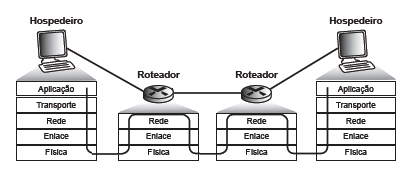
\includegraphics[width=300pt]{pilha-protocolo.png}
    \caption{Fluxo de dados (encapsulamente/desencapsulamento) na pilha de protocolos da Internet.  \cite[Adaptado]{KR09}}
    \label{fig:pilha_protocolos}
    \end{center}
\end{figure}



%\par Podemos notar nessa figura também que a complexidade dos nós é maior na borda (onde residem os sistemas finais) e menor no núcleo da Internet (onde se encontram os dispositivos responsáveis por processar os pacotes).
%\par Como já constatado em  \cite[p. 37]{KR09}, essas camadas, e os protocolos que fazem parte de cada uma delas, podem ser implementados em software, em hardware ou em uma combinação de ambas as abordagens. Assim como qualquer software ou circuito eletrônico, há inúmeras possibilidades que atingem um mesmo objetivo. Dessa maneira, diferentes desenvolvedores de softwares e fabricantes de equipamentos responsáveis por executar os protocolos de comunicação que regem o funcionamento da Internet têm desenvolvido diferentes soluções para tal. O interessante desse aspecto é que a continua competitividade do mercado e a constante busca por alto desempenho, tornaram os equipamentos presentes no núcleo da Internet extremamente fechados. A implementação da pilha de protocolos nos equipamentos, em geral, é conhecida somente pelo fabricante, e quando não é, essa implementação é realizada em uma combinação de software e hardware de tal modo inseparável que é impraticável realizar qualquer mudança no modo de operação do equipamento. Isso torna a rede fechada para experimentações e pesquisas de novos protocolos, pois há inúmeros sistemas críticos em operação na Internet que não podem sem interrompidos, dificultando a melhora dos protocolos existentes, desenvolvimentos de novos protocolos ou até mesmo desenvolvimento de novos tipos de redes. Devido a esses fatores que a Internet tem se tornado "ossificada"  e o paradigma das Redes Definidas por Software vem de encontro com essa necessidade que há de um ambiente mais flexível. Ambiente esse onde hája espaço para experimentações e mudanças em conjunto com uma rede em funcionamento normal que não pode ter seus fluxos de dados afetados por experimentações.


Como discutido por \citeonline[p. 37]{KR09}, as camadas e os protocolos que fazem parte de cada uma delas podem ser implementados em software, em hardware ou em uma combinação de ambas as abordagens. Assim como qualquer software ou circuito eletrônico, há diversas possibilidades de implementação que podem atingir um mesmo objetivo. Dessa maneira, diferentes desenvolvedores de softwares e fabricantes de equipamentos responsáveis por executar os protocolos de comunicação que regem o funcionamento da Internet têm desenvolvido diferentes soluções para tal. O interessante desse aspecto é que a especificação de protocolos da pilha é tal que permite a interoperabilidade entre dois sistemas finais (Windows e Linux, por exemplo), mesmo cada um tendo uma implementação específica desses protocolos de acordo com o sistema operacional.

%@FS: Esse parágrafo ficará para semestre que vem... Essa semana ta puxada (14/11/12)
\begin{comment}  \bkc{(refazer esse parágrafo ... o problema não é o equipamento ser fechado, mas sim a própria definição da operação da pilha (complexo na borda com os sistemas finais e muito simples/enxuto no núcleo da rede), que é ossificada/enrijecida ... inviabilizando modificações)} 
\end{comment}
%Devido a esses fatores que a Internet tem se tornado "ossificada"  e o paradigma das Redes Definidas por Software vem de encontro com essa necessidade que há de um ambiente mais flexível. Ambiente esse onde hája espaço para experimentações e mudanças em conjunto com uma rede em funcionamento normal que não pode ter seus fluxos de dados afetados por experimentações.

Por um lado, as decisões de projeto quanto à arquitetura da Internet a tornaram robusta e escalável para atender enorme demanda de dispositivos na rede que cresce exponencialmente ao longo dos anos; por outro lado, a operação pouco flexível da pilha TCP/IP tornou essa arquitetura ``ossificada''. O paradigma das Redes Definidas por Software vem ao encontro da necessidade das aplicações atuais, que demandam requisitos que são melhores atendidos a partir de um ambiente de rede mais flexível. Ambiente esse onde haja espaço para experimentações e mudanças no controle da rede para manipulação de novos fluxos, mantendo normalmente a operação da pilha sem que as transmissões dos dados das aplicações sejam afetados pela inserção de novos fluxos na rede.


%\par Não serão aprofundados por esse trabalho os protocolos presentes nas camadas físicas, de enlace e camada de aplicação. O objetivo desse trabalho é analisar o problema da mobilidade de nós finais na Internet, de forma que o foco estará sobre os protocolos responsáveis por identificar e localizar nós na rede e na forma como esses nós interagem com outros nós e com a rede em si. Os protocolos responsáveis por tais tarefas residem nas camada de rede e camada de transporte. Na camada de rede, o protocolo dominante na Internet é o protocolo IP \cite{rfc791}, já na camada de transporte os protocolos TCP\cite{rfc793} e UDP \cite{rfc768} são os mais largamente utilizados. Desses dois, o protocolo IP é principal alvo desse trabalho.

Não serão aprofundados por esse trabalho os protocolos presentes nas camadas físicas, de enlace e camada de aplicação. O objetivo desse trabalho é analisar o problema da mobilidade de sistemas finais na Internet, de forma que o foco estará sobre os protocolos responsáveis por identificar e localizar nós na rede e na forma como os mesmos interagem com outros nós e com a rede em si. Os principais protocolos nesse contexto residem nas camada de rede e camada de transporte. Na camada de rede, o protocolo dominante na Internet é o protocolo IP~\cite{rfc791}. Já na camada de transporte, os protocolos TCP~\cite{rfc793} e UDP~\cite{rfc768} são de fato os protocolos largamente utilizados pelos sistemas finais. Dentre os protocolos nessas duas camadas, o protocolo IP na camada de rede é o principal alvo desse trabalho.

\subsection{Protocolo IP}

%@FS{
%   Pretendo inserir aqui uma subseção: Internet Protocol - IP e então enriquecer o texto abaixo.

%   falta mencionar:
%    - Versões diferentes IPv4 IPv6
%    - Internet -> comutação de pacotes
%    -
%   inserir figura cabeçalho IPv4/IPv6
%   Explicar melhor o endereçamento IP (Fundamental)
%}
%\subsection{Endereçamento IP}
%\par O protocolo IP é o protocolo  responsável pelo controle das conexões e portanto, têm um importante papel no modo como funciona a Internet de hoje. Para que se entenda melhor o problema que um sistema final sofre ao trocar de rede, é necessário entender como se dá o endereçamento desses sistemas finais na camada de Rede.

O protocolo IP (\textit{Internet Protocol}~\cite{rfc791} é  responsável pela localização e identificação dos nós na Internet e, portanto, tem um importante papel no modo como a rede mundial opera. Para que se entenda melhor o impacto que um sistema final sofre ao trocar de rede IP, é necessário entender como ocorre o endereçamento desses sistemas finais na camada de rede. No contexto do endereçamento, há poucas diferenças de operação entre as diferentes versões do protocolo IP. Somado a esse, está o fato de que o IPv4 é a versão do protocolo ainda amplamente utilizada. Desse modo, através do esclarecimento da operação do IPv4, é possível extender o esclarecimento para o IPv6.

A Internet é uma rede de comutação de pacotes. Isso significa que os dados que trafegam por ela são segmentados em pacotes que são processados individualmente durante as operações de repasse e roteamento. Cada segmento recebe uma denominação de acordo com a camada da rede que faz parte, desse modo, um pacote da camada de rede é denominado datagrama IP. Um datagrama IP é constituído de um cabeçalho e de uma carga útil. A carga útil é a porção do datagrama referente aos dados de interesse das camadas acima da camada de rede. O cabeçalho é a porção do datagrama onde constam as informações necessárias ao processamento desse datagrama pelos elementos de rede. Os campos de um datagrama IPv4 são apresentados na Figura~\ref{fig:cabecalho_IPv4} e suas principais funções são as seguintes:

\begin{figure}[ht!]
    \begin{center}  
    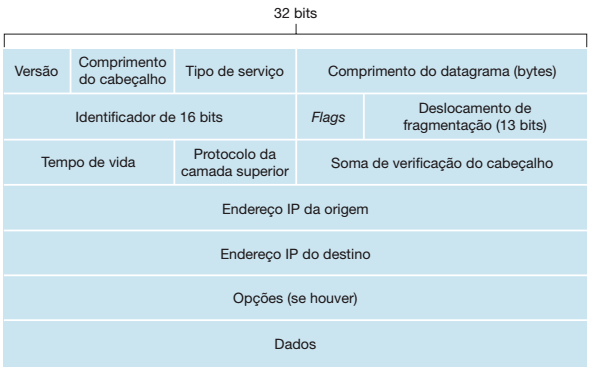
\includegraphics[width=400pt]{cabecalho-IP.png}
    \caption{Protocolo IP - Cabeçalho IPv4 .  \cite{kurose2013computer}}
    \label{fig:cabecalho_IPv4}
    \end{center}
\end{figure}

\begin{itemize}
    \item{\textbf{versão}}, quatro bits que sinalizam a versão do protocolo IP. Utilizado para determinação de como processar o restante do datagrama.
    \item{\textbf{Comprimento do cabeçalho}}, o cabeçalho de um datagrama  IPv4 possui 20 bytes que são fixos. O campo opções, se utilizado, acarreta em aumento desse valor, de modo que é necessário informar o tamanho do cabeçalho para que o elemento que está processando esse datagrama saiba onde termina o cabeçalho e onde começam os dados. Este campo consiste de quatro bits.
    \item{\textbf{Tipo de Serviço}}, oito bits utilizados para informar a que tipo de serviço os dados desse datagrama corresponde. Por exemplo, através desse campo pode-se distinguir datagramas de tempo real de tráfego que não é de tempo real.
    \item{\textbf{Comprimento do datagrama}}, são 16 bits utilizados para informar o comprimento total do datagrama em bytes. Com esses 16 bits pode-se representar 65.535 bytes, porém, dificilmente um datagrama IP possui tamanho maior do que 1500 bytes. Ainda assim, esses datagramas podem ter tamanho menor do que 1500 bytes, geralmente no ultimo datagrama de um transmissão, de modo que com esse campo pode-se calcular onde o datagrama termina.
    \item{\textbf{Identificador de 16 bits, flags, deslocamento de fragmentação}}, datagramas IP podem ser fragmentados em datagramas menores. Esses campos são utilizados quando isso ocorre.
    \item{\textbf{Tempo de vida}}, são oito bits que dizem o tempo que um pacote deve sobreviver na rede. Esse tempo é medido em saltos, i.e., toda vez que um elemento de rede processa esse datagrama, o valor desse campo é decrementado em uma unidade. Utilizado para que um datagrama não fique eternamente circulando na rede. Quando o valor desse campo chega a zero, ele é descartado.
    \item{\textbf{Protocolo da camada superior}}, quando um datagrama termina de ser processado na camada de rede, deve ser encaminhado ao protocolo de camada de transporte adequado. Esse campo é utilizado para informar a qual protocolo ele deve ser encaminhado. É um campo de ligação entre as camada de rede e de transporte.
    \item{\textbf{Soma de verificação do cabeçalho}}, campo utilizado para auxiliar na verificação de erros no cabeçalho do datagrama em questão. Esse valor é calculado da seguinte maneira: a cada 2 bytes do cabeçalho são obtidos valores decimais correspondentes. Esses valores são somados utilizando complementos aritméticos de 1. O complemento de 1 dessa soma é então armazenado nesse campo. Toda vez que um roteador vai processar um datagrama, primeiramente ele irá calcular essa soma e comparar com o valor desse campo, se os valores forem diferentes, ele assume que há um erro e descarta o datagrama.
    \item{\textbf{Endereço IP da origem}}, um elemento qualquer de uma rede, quando cria um datagrama necessita colocar seu endereço nesse campo de 32 bits. O endereço de um sistema final é determinado da seguinte maneira: a cada 8 bits é obtido um número decimal equivalente, de modo que o endereço de um nó consiste de 4 números decimais de 0 a 255. 
    \item{\textbf{Endereço IP do destino}}, análogo ao campo IP de origem, nesse campo de 32 bits é inserido o endereço IP do destinatário do datagrama.
    \item{\textbf{Opções}}, campo de 32 bits que permite a extensão do cabeçalho IP. Raramente é utilizado, tal que na versão 6 não existe esse campo.
    \item{\textbf{Dados}}, Corresponde à carga útil do datagrama IP, os dados de interesse que estão sendo transmitidos pela rede.
\end{itemize}


%\par À cada dispositivo conectado à Internet, através dos mecanismos apropriados, é atribuído um identificador único em formato numérico específico denominado número IP. Esse identificador permite à rede localizar e distinguir um dispositivo dos demais, e assim, entregar à ele os pacotes que lhe são transmitidos. A distribuição dos números IPs se dá de forma hierarquizada, de modo que um pacote que sai de um nó final na borda da Internet, possa ser rapidamente processado conforme vai subindo na hierarquia, e assim este pacote vai sendo direcionado para diferentes redes de destino, até que atinja o nó de borda final alvo \cite{rfc791}. 

Para esse trabalho, os campos de maior interesse são os de Endereço IP do destino e Endereço IP de origem. Como visto, o endereço IP consiste de um campo de 32 bits, que equivale a 4 bytes. Por convenção, esse endereço é apresentado em notação decimal separada por pontos, i.e., cada byte é escrito em seu valor decimal equivalente, separado dos outros bytes por um ponto. Por exemplo, 123.1.2.3 é um endereço IP em notação decimal, em sua notação binária ele é escrito 01111011.00000001.00000010.00000011. É interessante saber como é o endereço IP em sua notação binária para entender como cada endereço IP é atribuído e processado pelos nós de uma rede. Em uma rede comum, cada sistema final se conecta à rede através de uma, ou mais, interfaces de rede. Os meios pelos quais as interfaces de rede de diferentes sistemas finais estão conectados é denominado \textit{enlace}.

Uma vez que o dispositivo obtém acesso ao enlace (\textit{link}) de transmissão através dos mecanismos próprios de cada tecnologia, é necessário identificá-lo em rede através de um endereço IP único. Esse endereço permite localizar o dispositivo e saber a qual rede o mesmo pertence, bem como identificar esse dispositivo unicamente nessa rede, distinguindo-o de qualquer outro dispositivo de qualquer outra rede na Internet. Esse endereçamento, portanto, permite que os sistemas se comuniquem de forma fim-a-fim com o suporte de roteadores, que encaminham pacotes de dados endereçados unicamente com IPs de origem e destino. 

O endereço IP que cada dispositivo recebe é dependente da rede em que ele se encontra. Assim, uma rede também é identificada e localizada por um endereço IP único. Considere o endereço de uma rede 123.1.2.0/24. A notação /24 é denominada \textbf{máscara de sub-rede} e significa que todos os nós sob esta rede receberão endereços IPs únicos e distintos nos quais todos os 24 bits mais à esquerda são os mesmos. Dessa forma, qualquer sistema final nessa rede possuirá um endereço na forma 123.1.2.xxx. Observe que através do endereçamento IP um dispositivo pode ser localizado e identificado. Localizado pois um certo números de bits à esquerda explicita em qual rede ele se encontra, e identificado porque o endereço IP que ele possuí é único.


%\par Esse é modo como as transmissões de dados é realizada na Internet e a atribuição dos números IPs é o grande responsável também pelo problema da mobilidade. Como um dispositivo recebe um número de IP único de acordo com a rede na qual está conectado, se esse dispositivo sai de uma rede e se conecta em outra, lhe é atribuído um número IP distinto do primeiro que possuía. Issp deve ocorrer para que a hierarquia de endereços não seja violada, no entanto, todos os dados que eventualmente estavam em trânsito pela rede tendo como destino o primeiro número IP atribuído, não terão mais o destino conhecido para atingir e serão descartados pelos dispositivos intermediários da reded. Uma solução para esse problema de mobilidade deve tratar essa situação de modo que as conexões existentes não sejam perdidas quando um nó se move de uma rede para outra, e é desejado que o tratamento dessa solução seja realizado de modo transparente para a aplicação, e da forma menos custosa para os diversos dispositivos responsáveis por rotear os dados transmitidos pela Internet. Os estudos para atingir uma solução eficaz para esse problema são inúmeros como será visto na seção Trabalhos relacionados mas em todos eles o problema de se alterar a forma como a Internet de hoje é estruturada é bastante criticada o que, novamente, reforça os benefícios de se utilizar Redes Definidas por Software \cite{McKeown} para tratar o problema.

Esse modo como as transmissões de dados são realizadas na Internet e a semântica do endereço IP, que localiza e identifica o nó ao mesmo tempo, inviabilizam a mobilidade do nós sob transmissão em andamento entre diferentes rede acesso. Como um dispositivo recebe um endereço IP único da rede a qual está ligado, se esse dispositivo sai de uma rede e se conecta em outra, lhe é atribuído um número IP distinto do primeiro que possuía. 

Essa realocação de endereços deve ocorrer para que operação da rede, de roteamento e encaminhamento, não seja violada. No entanto, pacotes de dados que eventualmente estavam em trânsito para rede de destino definida pelo primeiro IP atribuído, não terão mais o destino disponível para atingir e serão descartados pelos dispositivos intermediários da rede, como roteadores e switches. Uma solução de mobilidade deve tratar essa situação de modo que as conexões estabelecidas pelas aplicações não sejam rompidas quando o nó se move de uma rede para outra. Idealmente, é desejável que o tratamento dessa solução seja realizado de modo transparente à operação da aplicação e da forma menos custosa possível para os diversos dispositivos responsáveis por rotear pacotes na Internet. Estudos que propõem soluções para esse problema são diversos, como serão vistos na seção Trabalhos relacionados mais adiante. Entretanto, grande parte das soluções propõe adaptações de protocolos legados da pilha nos sistemas finais e muitas vezes no núcleo da Internet, tornando as soluções custosas tanto do ponto de vista de manutenção quanto de implantação. Nesse contexto, Redes Definidas por Software \cite{McKeown}, embora impliquem num alto custo inicial de implantação da tecnologia devido a necessidade de equipamentos de interconexão compatíveis com protocolo OpenFlow, possui um custo muito baixo de manutenção e implantação de soluções de rede para tratar problemas que hoje são complexos pela pilha TCP/IP, como é o caso da mobilidade.

%@FS: Anotações, itens a serem citados:
% - Conexões sem fio
% - Power Management
\subsection{Computação Móvel}
%\par Historicamente, a computação surgiu em estações fixas, grandes máquinas que realizavam cálculos automaticamente através de uma prévia programação. Com o tempo, essas máquinas foram avançando em tecnologia e diminuindo em tamanho, mas ainda eram estações fixas quando do surgimento da Internet. Devido a isso a Internet, embora tenha sido um projeto muito bem elaborado inicialmente, principalmente em se tratando de escalabilidade, previa apenas nós estacionários nas rede. Mas com a miniaturização dos dispositivos, começaram a surgir os pequenos computadores que podiam ser levados para onde quer que as pessoas pudessem ir. O nascimento dessas tecnologias tornou aprazível o avanço nos meios de transmissão de dados via rádio, que já existia nos aparelhos celulares, mas que foram então interligadas com a Internet.

Historicamente, a Computação surgiu em estações fixas,  máquinas de grande porte que realizavam cálculos automaticamente através de uma prévia programação. Com o tempo, essas máquinas foram avançando em tecnologia de processamento e diminuindo em tamanho, mas ainda eram estações fixas quando do surgimento da Internet. Devido a isso a Internet, embora tenha sido um projeto muito bem elaborado inicialmente, principalmente em se tratando de escalabilidade, previa apenas nós estacionários nas redes. Com a miniaturização dos dispositivos, começaram a surgir os pequenos computadores pessoais que podiam ser levados para onde quer que as pessoas pudessem ir. O nascimento dessas tecnologias incentivou o avanço dos meios de transmissão de dados via rádio, que já existia nos aparelhos celulares para transmissão de voz em comutação por circuito, para então realizar comutação por pacotes de dados, permitindo que esses dispositivos fossem conectados na Internet.

%\par Com o advento das tecnologias sem fio houve um aumento significativo, tanto no número, quanto na diversidade de dispositivos que podem se conectar a Internet. Com isso, o número de aplicações que utilizam dessa recente tecnologia para oferecer os mais variados serviços para as pessoas, tem aumentado consideravelmente \cite{CISCO2017}. Tal fato culminou no surgimento de alguns termos bastante abstratos como é o caso da Computação Móvel \cite{mobilecomputing}. Em linhas gerais, o termo Computação Móvel faz referência a diversos princípios, métodos, tecnologias, que envolvem os serviços oferecidos através dos novos meios de transmissão de dados, particularmente aqueles que permitem aos usuários se conectar à Internet de forma tão diversificada e, principalmente, móvel.

Com o advento das tecnologias de comunicação sem fio houve um aumento significativo, tanto no número, quanto na diversidade de dispositivos que podem se conectar a Internet. Com isso, o número de aplicações que utilizam a rede mundial para oferecer os mais variados serviços para as pessoas tem aumentado consideravelmente~\cite{CISCO2017}. Tal fato culminou no surgimento de um novo paradigma em Computação denominado \textbf{Computação Móvel}~\cite{mobilecomputing}. Esse paradigma faz referência aos diversos princípios, métodos e tecnologias que envolvem o oferecimento de serviços em ambiente computacional através de meios de transmissão sem fio de dados. Particularmente, esses meios de transmissão devem permitir que usuários se locomovam enquanto exercem atividades em ambiente computacional através de dispositivos portáteis, implicando, muitas vezes, em estarem conectados à Internet de forma diversificada.


%\par Essa preocupação  não é tão recente assim. Em \cite{mobilecomputing} é apresentado uma vasta discussão sobre o assunto, e tal documento foi publicado em 1996. Embora o termo naquela época pudesse ser considerado recente, o assunto já era discutido em outras literaturas como Computação Nômade, ou ainda Computação Ubíqua. Esses termos tratam da capacidade que as pessoas têm hoje, de acessar os mais diversos serviços presentes na Internet, de onde quer que estejam, seja utilizando seus \textit{smartphones, laptops, notebooks}, ou qualquer de inúmeros outros dispositivos portáteis.

O paradigma não é recente e aparece na literatura há mais de duas décadas~\cite{mobilecomputing}. Embora o termo Computação Móvel seja hoje bem compreendido, naquela época era abstrato e muitas vezes discutido e referenciado de outras formas na literatura, como \textbf{Computação Nômade}, ou ainda \textbf{Computação Ubíqua e Pervasiva}. Esses termos são mais especializados e se referem à facilidade que as pessoas têm hoje de acessar os mais diversos recursos disponíveis na Internet, de onde quer que estejam, a qualquer momento,  utilizando qualquer dispositivo portátil, como  \textit{smartphones}, \textit{laptops}, \textit{notebooks}, \textit{tablets}, \textit{smart watches}, etc \cite{rouse2007nomadic} e \cite{lyytinen2002ubiquitous}. 
%\bkc{(buscar referência que suporte essa afirmação)}


\begin{comment}
\bko{Em sua grande maioria, os princípios da Computação Móvel são mais objetos de desejo do que funcionalidades oferecidas de forma fácil pela Internet. Assim o é o caso de algumas aplicações que oferecem suporte a mobilidade, mas tratando-a na camada da aplicação, já que a Internet de hoje ainda não oferece esse tipo de serviço \cite{mobilecomputing}. Isso faz com que a carga de processamento dos dispositivos seja aumentada, visto que o próprio dispositivo tem que que estar a todo momento verificando alterações na rede em que se encontra. Quando o dispositivo observa alteração na rede, ele deve realizar as tarefas necessárias para que as aplicações que estão utilizando os serviços da Internet não entrem em colapso. Na verdade, cada aplicação é que faz essa verificação, o que é ainda pior, pois a carga de processamento do dispositivo é proporcional ao número de aplicações em execução, o que diminui consideravelmente o tempo de carga da bateria do dispositivo.} \bkc{(refazer este parágrafo ou remover. começa falando de princípios que não foram apresentados ... depois fala da mobilidade na aplicação que é custosa em processamento e energia, mas não apresenta nenhuma referência para suportar essa afirmação ... daí parece ``achismo'', coisa que deve ser evitada em texto acadêmico ...)}

%\par Tornar a rede capaz de tratar a mobilidade desses sistemas finais irá retirar das aplicações uma carga de trabalho muito grande, tornando-as mais leves e menos complexas. Com isso, pode se obter uma diminuição na carga de trabalho das aplicações, indiretamente, isso resultará em uma diminuição no número de mensagens de controle que as aplicações devem trocar para tratar sua própria mobilidade. Tal fator é desejável também por parte da rede, pois diminuindo o número de mensagens que são trocadas entre dispositivos, aumenta a largura de banda disponível para realizar envio e recebimento de mensagens "úteis" para cada aplicação.

\bko{Tornar a rede capaz de tratar a mobilidade desses sistemas finais irá retirar das aplicações uma carga de trabalho muito grande, tornando-as mais leves e menos complexas. Com isso, pode se obter uma diminuição na carga de trabalho das aplicações, indiretamente, isso resultará em uma diminuição no número de mensagens de controle que as aplicações devem trocar para tratar sua própria mobilidade. Tal fator é desejável também por parte da rede, pois diminuindo o número de mensagens que são trocadas entre dispositivos, aumenta a largura de banda disponível para realizar envio e recebimento de mensagens "úteis" para cada aplicação.} \bkc{(De onde tirou isso??? Tem alguma ref??? A sobrecarga de mensagem de controle de mobilidade na aplicação costuma ser irrisória (algumas centenas bytes somente no estabelecimento de (re)conexões ...) o que não onera a rede)}
\end{comment}
%Tem um capitulo do livro "Mobile Computing" que trata do assunto ( cap 3).
%
%How does the network know where a given user is? How does the network route messages to mobile users?
%Duas comunidades diferentes: Internet e Cellular-communities
%searching and informing (pg 18)

\subsection{Gerenciamento de Mobilidade}

%\par Foi visto que a Internet, em sua criação, não foi construída prevendo que sistemas finais pudessem se mover no espaço e, consequentemente, entre redes distintas. Com isso, se tem hoje uma dificuldade para tratar desses sistemas finais móveis, que existem e não são poucos \cite{CISCO2017}. Uma das principais características da Internet que torna tal tratamento difícil se encontra na camada de rede, a grande responsável por realizar repasse e roteamento, tarefas fundamentais na Internet, pois nela é utilizado o protocolo IP como mecanismo principal nessas atividades de processamento dos pacotes. O protocolo IP utiliza o endereço IP atribuído a cada nó tanto para localização como para identificação. Essa dupla semântica do protocolo IP torna o controle dos nós complexo pois a mudança de localização acarreta na mudança de IP, ou seja, quando um sistema final, por algum motivo, deseja se desconectar de um dada rede e se conectar a outra, ele receberá dessa nova rede um novo número IP de acordo com o prefixo dessa nova rede. Como então a rede irá saber onde um nó específico se encontra se sua identificação muda constantemente? Como a rede irá enviar pacotes para um nó que se move constantemente entre redes distintas? Nesse contexto, surge a necessidade da aplicação de técnicas e métodos que auxiliem no tratamento da mobilidade desses sistemas finais, o conjunto dessas técnicas e métodos utilizados para esse fim são denominados Gerenciamento de Mobilidade \cite{pandya2004}.

Como introduzido anteriormente, a arquitetura da Internet, em seu projeto, não havia sido previsto que os nós iriam se comunicar via transmissor de rádio, tampouco se mover entre redes distintas de acesso sem fio. Com isso, se tem hoje um complexo mecanismo para tratar a comunicação desses sistemas finais móveis, que não são poucos~\cite{CISCO2017}. Uma das principais características da Internet que torna tal tratamento difícil se encontra na camada de rede,  responsável por realizar repasse e roteamento, tarefas fundamentais na Internet. Nessa camada é utilizado o protocolo IP como mecanismo principal para o processamento dos pacotes. 

O protocolo IP define o endereço de tal forma que é utilizado tanto para localizar quanto para identificar o nó. Essa semântica dúbia no endereçamento do protocolo IP torna o controle dos nós móveis complexo, pois a mudança de localização acarreta na mudança de IP, ou seja, quando um sistema final, por algum motivo, deixa uma rede e se conecta a outra, o mesmo receberá em sua nova localização um novo endereço IP de acordo com o prefixo dessa nova rede. Como então a rede irá saber onde um nó específico se encontra se sua identificação muda? Como a rede irá enviar pacotes para um nó que se move entre redes distintas? Nesse contexto, surge a necessidade da aplicação de técnicas e métodos que auxiliem no tratamento da mobilidade desses sistemas finais. O conjunto dessas técnicas e métodos utilizados para esse fim são denominados Gerenciamento de Mobilidade~\cite{pandya2004}.

%\par O conceito de mobilidade é largamente empregado e faz referência a capacidade de um nó se mover entre redes distintas sem perder as conexões lógicas previamente estabelecidas, como já foi dito. Desde a publicação da RFC 2002 \cite{perkins1996} o termo tem sido utilizado e bastante discutido e o modo como é realizado o Gerenciamento da Mobilidade é até mesmo usado para sua classificação em algumas literaturas \cite{pandya2004}.

O conceito de suporte à mobilidade tem sido amplamente empregado no sentido de qualificar a capacidade de um nó se mover entre redes distintas sem perder as conexões lógicas estabelecidas em redes prévias. Desde a especificação do padrão RFC~2002~\cite{perkins1996}, o tema de mobilidade na Internet tem sido bastante explorado ao longo dos anos, tornando-se maduro ao ponto de existir classificações do suporte provido pelas soluções~\cite{pandya2004}. \citeonline{pandya2004} propõe a seguinte classificação:
%\par Algumas das classificações apresentadas em \cite{pandya2004}, são:
\begin{itemize}
%    \item{\textbf{Portabilidade de Serviços}}
%    \par Esse tipo também pode ser referenciado como Mobilidade de Seção e é aquele que prevê quem um indivíduo pode manter suas seções ativas mesmo realizando trocas de dispositivo, não é parte do escopo desse trabalho, pois tal tratamento envolve grande parte da própria aplicação.
    \item \textbf{Portabilidade de Serviços}. Esse tipo de suporte à mobilidade também pode ser definida como Mobilidade de Sessão, que é aquela que prevê que o usuário mantenha suas sessões ativas mesmo realizando trocas de dispositivo. Por exemplo, uma sessão de videoconferência é migrada do \textit{smartphone} para o notebook de forma transparente para o usuário, sem qualquer necessidade de intervenção do mesmo, a não ser a indicação do dispositivo alvo para continuar a sessão. Esse tipo de mobilidade não é parte do escopo deste trabalho.
    
%    \item{\textbf{Mobilidade Pessoal}}
%    \par Esse tipo de tratamento de mobilidade prevê que cada usuário final manterá um único identificador global o qual poderá ser utilizado pelo usuário para iniciar sessões de qualquer dispositivo que desejar. O mesmo identificador também será utilizado pela rede para o localizar. Também não fara parte do escopo desse trabalho dado que não será considerado que cada indivíduo poderá manter um único identificador imutável pois se isso fosse levado para a camada de rede, deverá ser reformulado o protocolo IP já que a identificação de um nó em determinada sub-rede depende diretamente da sub-rede à que esse nó está conectado. 

    \item \textbf{Mobilidade Pessoal}. Esse tipo de tratamento de mobilidade prevê que cada usuário possa ser globalmente alcançável através de um identificador global único, através do qual ele é capaz de iniciar e/ou aceitar sessões de qualquer dispositivo. Também não fará parte do escopo deste trabalho esse tipo de mobilidade. 
    
%    \item{\textbf{Mobilidade de Terminal}}
%    \par Aqui a palavra terminal é utilizada para referenciar o próprio dispositivo que está sendo utilizado. Esse tipo de tratamento de mobilidade se refere aquele que oferece ao usuário, ou ao sistema final em questão, a possibilidade de se mover para sub-redes distintas e ainda assim manter suas conexões lógicas previamente estabelecidas ativas. Dessa maneira, ele continuará tendo acesso ininterrupto aos serviços utilizados ao mesmo tempo em que pode ser "localizado" por outros sistemas finais que conheciam sua identificação em algum momento antes da troca de sub-rede. Repare que nesse tipo de tratamento não há nenhuma restrição quanto a manter, ou não, a identificação do usuário imutável, após a troca de rede. 
   \item \textbf{Mobilidade de Terminal}. Aqui a palavra terminal é utilizada para referenciar o próprio dispositivo que está sendo utilizado e migrado pelo usuário. Esse tipo de tratamento de mobilidade se refere aquele que oferece ao usuário, tecnicamente às aplicações em execução no sistema final em questão, a possibilidade de se mover para redes distintas e ainda assim manter ativas as suas conexões lógicas previamente estabelecidas. Dessa maneira, o usuário continuará tendo acesso ininterrupto aos serviços em uso e as transmissões em andamento de grande volume de dados, como download/upload de conteúdo. 

\end{itemize}

%\par O tratamento da Mobilidade de Terminal é o tipo que irá ser tratado nesse trabalho. Nesse tipo de tratamento estão aquelas soluções que, ao serem empregadas, tornam a rede capaz de lidar com a mobilidade dos nós. Com a rede tendo a responsabilidade de tratar a mobilidade dos nós, as aplicações, e os próprios dispositivos, estarão livres de se preocupar com alterações nas conexões lógicas estabelecidas. É como se houvesse uma camada na pilha de protocolo responsável por oferecer esse serviço à camada superior. Nessa analogia, a camada que oferece esse serviço estaria implementada somente nos elementos de rede.

Mobilidade de Terminal é o objeto de estudo neste trabalho. Particularmente,  o foco será na investigação de soluções que, ao serem empregadas, tornam a rede capaz de lidar com a mobilidade de seus nós. Com a rede tendo a responsabilidade de tratar a mobilidade dos nós, as aplicações, e os próprios dispositivos, estarão livres de se preocupar com alterações nas conexões lógicas estabelecidas. É como se houvesse uma camada na pilha de protocolo responsável por oferecer esse serviço à camada superior. Contudo, a camada que oferece esse serviço estaria implementada somente nos elementos de rede.

%@FS: Melhorar esse parágrafo.Não está legal.
%\par A IETF tem se esforçado para inserir no modelo TCP/IP algum suporte para mobilidade. Tal esforço pode ser notado através das publicações das RFCs 3220  \cite{rfc3220} e 3775 \cite{rfc3775}, que definem suporte para mobilidade sobre o protocolo IPv4 e IPv6, respectivamente. No entanto, nenhuma dessas soluções é viável, considerando que para implantação dessas melhorias seria necessário realizar mudanças na infraestrutura da Internet. Neste trabalho irá se focar nas soluções que exijam o mínimo de alteração na infraestrutura da Internet de hoje, pois, como discutido em \cite{raychaudhuri2012}, uma solução como a proposta por \cite{rfc3775} é custosa demais para ser implantada, dado que o modo de operação que sugere é incompatível com o modo atual, ou seja, para implantação dessa solução, seria necessário interromper, ou reescrever, a grande maioria dos serviços que rodam atualmente na Internet. Desse modo, uma vez realizada a mudança, os antigos serviços não mais funcionariam. Como tal procedimento não é viável, a busca por uma nova Internet, com maior flexibilidade, se tornou um amplo campo de pesquisas, no qual novas tecnologias tem surgido, uma delas: o paradigma das Redes Definidadas por Software que será descrito na próxima seção.

Ao longo das últimas duas décadas, a IETF tem publicado diferentes soluções para tratar mobilidade na pilha TCP/IP. O IP Móvel (\textit{Mobile IP}) foi o primeiro protocolo a ser especificado. As RFCs~3220~\cite{rfc3220} e 3775~\cite{rfc3775} que definem suporte à mobilidade do protocolo IP Móvel para redes IPv4 e IPv6, respectivamente. Essa solução, embora muito bem idealizada, apresenta custo elevado de implantação e manutenção. Ao necessitar de mudanças tanto na pilha de protocolos dos nós envolvidos na comunicação fim-a-fim quanto na infraestrutura de redes de acesso e do núcleo da Internet, o IP Móvel tem pouca viabilidade. 

%%%%%%%%%%%%%%   REVER     %%%%%%%%%%%%
\begin{comment}
\bko{Como discutido por \citeonline{raychaudhuri2012}, o custo é elevado, pois sugere modo de operação incompatível com o modo atual, ou seja, para implantação dessa solução, seria necessário interromper, ou reescrever, a grande maioria dos serviços que rodam atualmente na Internet. Desse modo, uma vez realizada a mudança, os antigos serviços não mais funcionariam.} \bkc{(rever essa afirmação... o ip móvel é proposto na camada de rede justamente para ser transparente e não demandar nenhuma alteração nas aplicações/serviços ...)}
\end{comment}

Dado a complexidade de se atender requisitos das aplicações com soluções sobre a pilha de protocolos existente, a busca por uma nova Internet, de maior flexibilidade, se tornou um amplo campo de pesquisa, o qual induziu o surgimento das Redes Definidas por Software como  novo paradigma de gerenciamento e operação de redes de computadores. Nesse contexto, este trabalho irá focar em soluções de mobilidade que sejam menos custosas nas etapas previstas de implantação e ou manutenção através da flexibilidade proporcionada por Redes Definidas por Software.

\subsection{Redes Definidas por Software}

%\par Apesar do grande sucesso que a Internet atingiu, fato que pode ser constatado observando sua presença em todo tipo de atividade no cotidiano das pessoas, essa tecnologia atingiu um estado de maturidade considerado pela comunidade de pesquisadores  como "calcificada" \ (ou "ossificada") \cite{Zhang2010}. Tal consideração se dá pela dificuldade que se tem em realizar mudanças no modo como a Internet funciona. Essa dificuldade ocorre pois em todos os níveis de sua infraestrutura são utilizados elementos de redes que operam com softwares fechados sobre hardwares proprietários. Assim, a utilização de novas tecnologias quase sempre exige troca do hardware, o que é inviável dada a escala global da utilização da Internet. Com isso, os novos problemas que têm surgido com o aumento da diversidade de tecnologias dos dispositivos presentes na Internet, penam em encontrar soluções eficientes e definitivas. Ainda que soluções sejam desenvolvidas, não são aplicadas, porque encontram dificuldades para serem testadas em ambiente real, além do que seria necessário realizar troca dos elementos de rede no mundo todo para sua adoção. O conjunto desses fatores (a "ossificação" da Internet e o surgimento de novas necessidades) semeou o surgimento de um novo paradigma que flexibilizou a maneira como os fluxos de dados são tratados em uma rede de computador: o paradigma das Redes Definidas por Softwares (SDN - Software Defined Network) \cite{McKeown}.

A facilidade do acesso e a crescente disponibilidade de serviços na Web levaram a um estilo de vida moderna, onde as pessoas são cada mais dependentes da Internet. Tal fato pode ser constatado, observando a necessidade de acesso à Internet em atividade mais diversas do cotidiano das pessoas. Entretanto, a Internet, particularmente as tecnologias que a suportam através da pilha TCP/IP, atingiu um estado de maturidade considerado pela comunidade acadêmica  como ``calcificada'' ou ``ossificada''~\cite{Zhang2010}. Tal estado se dá pela dificuldade que se tem em realizar mudanças no modo como a Internet opera. Essa dificuldade ocorre, pois, em especial, as camadas de rede e transporte são implementadas nos sistemas finais e nos elementos intermediários (comutadores, roteadores, firewalls) por um conjunto muito restrito de protocolos composto pelo IP, TCP, UDP. As aplicações e a operação da rede ficam restritas apenas aos serviços providos por esses protocolos, tornando arquitetura da Internet inflexível à mudanças, como por exemplo: identificação única dos elementos, localização de nós móveis, formas de comunicação entre processos, interferência dos sistemas finais na decisão de encaminhamento dos pacotes.

Nesse contexto, a utilização de novas tecnologias muitas vezes exige a troca de componentes de hardware, o que é inviável na escala global de utilização da Internet. Com isso, problemas que têm surgido com o aumento do volume de dados pela diversidade de nós (ou coisas) conectadas à Internet, mas principalmente pelos os novos requisitos das aplicações dos usuários, encontrar soluções eficientes e definitivas na atual pilha de protocolos TCP/IP é um grande desafio. Ainda que soluções sejam desenvolvidas, muitas vezes não podem ser adotadas devido as dificuldades de serem testadas e implantadas em ambiente de larga escala como a Internet. Por exemplo, uma nova solução de camada de rede para Internet necessitaria de ser suportada por todos os comutadores e roteadores na rede mundial.

%\par Como o grande problema é a realização de mudanças, pesquisadores em Redes de Computadores tem buscado tornar os elementos de redes mais flexíveis. Buscam a flexibilidade no sentido de que a inserção  de novas tecnologias possa acontecer aos poucos e de maneira que novas tecnologias possam coexistir com as antigas. Atingindo esse objetivo, aqueles que relutarem em realizar alterações em suas redes não serão penalizados e nem irão atrapalhar a evolução da Internet como um todo. 

Uma vez que o maior problema da ``ossificação'' da pilha  é o impacto da realização de mudanças na rede, pesquisadores tem buscado tornar os elementos de redes mais flexíveis. Tal flexibilidade é almejada no sentido de que a inserção  de novas tecnologias possa acontecer gradativamente, de maneira que novas tecnologias possam coexistir com as já implantadas. Assim, protocolos legados que não podem sofrer alterações não serão penalizados e nem irão impedir a evolução da Internet. Nesse contexto, o conjunto de fatores (a pilha inflexível aos novos requisitos de aplicações) semeou o surgimento do novo paradigma de Redes Definidas por Softwares (SDN)~\cite{McKeown}, de modo a flexibilizar a maneira como os fluxos de dados são transmitidos em rede de comutação por pacotes.


%\par Os equipamentos utilizados para funcionamento da Internet necessitam de alto desempenho na tarefa de encaminhar pacotes, esse desempenho é alcançado através da combinação de circuitos dedicados especializados nesse tipo de processamento. Esse hardware é complementado por uma implementação em software que concede apoio em controlar o processamentos dos pacotes. A presença do software é necessária para que haja suporte a grande pilha de protocolos existente. O software é responsável por processar os pacotes e dizer ao hardware para onde cada pacote deve ser encaminhado. Esse software pode ser configurado através de interfaces conhecidas, porém são limitadas às funcionalidades programadas pelo fabricante do equipamento, como o software é fechado e integrado ao hardware, alterações estão sujeitas ao ciclo de desenvolvimento do fabricante do equipamento, os quais, para protegerem seus investimentos, mantêm fechadas as arquiteturas desses equipamentos. Note, no entanto, que essa arquitetura de roteamento de pacotes pode ser divida em duas camadas bem distintas: o hardware de alto desempenho, responsável por realizar encaminhamento de pacotes, e o software de controle, responsável pela tomada de decisão. Combinando essa constatação com a observação de que a tarefa que exige alto desempenho é a tarefa de encaminhar os pacotes, pesquisadores começaram a trabalhar em ideias que permitissem mover parte dessa lógica de controle para elementos externos aos elementos de roteamento da rede, mas de forma que a operação de encaminhamento de pacotes continuasse pouco alterada.

Os equipamentos utilizados para funcionamento da Internet necessitam de alto desempenho na tarefa de encaminhar pacotes. Esse desempenho é alcançado através da combinação de circuitos dedicados e específicos para esse tipo de processamento. O hardware então é complementado por uma implementação em software, o qual concede apoio em controlar o processamentos dos pacotes. A presença do software é necessária para que haja suporte à pilha de protocolos. O software é responsável por processar os pacotes e atribuir ao hardware a tarefa de onde cada pacote deve ser encaminhado. Esse software pode ser configurado através de interfaces conhecidas, porém são limitadas às funcionalidades programadas pelo fabricante do equipamento. Como o software é fechado e integrado ao hardware, alterações estão sujeitas ao ciclo de desenvolvimento do fabricante do equipamento, os quais, para protegerem seus investimentos, mantêm fechadas as arquiteturas de seus dispositivos. Note, no entanto, que a arquitetura de comutadores e roteadores de pacotes pode ser divida em duas camadas bem distintas: o hardware de alto desempenho, responsável por realizar encaminhamento de pacotes; e o software de controle, responsável pela tomada de decisão de/para onde encaminhar. Conhecendo a operação desses elementos e tendo a constatação de que a tarefa que exige alto desempenho é o encaminhamento de pacotes, pesquisadores começaram a vislumbrar ideias que permitissem mover parte dessa lógica de controle para elementos externos aos elementos de roteamento da rede, contudo, de forma que a operação de encaminhamento de pacotes continuasse pouco alterada.

%\par Assim começaram as iniciativas para tornar a rede mais programável e menos escravas das funcionalidades implementadas pelos fabricantes. Separando o plano de dados, isto é, a camada responsável por realizar o encaminhamento dos pacotes, do plano de controle, é possível manter o desenvolvimento desses hardwares independente do controle dos fluxos de dados. Assim, é possível oferecer maior controle por parte dos administradores e pesquisadores de redes, flexibilizando a inserção de novas tecnologias gradualmente \cite{guedes2012}. Uma tecnologia pioneira na qual essa ideia é inspirada é o encaminhamento de pacotes baseado em rótulos programáveis, como utilizado no MPLS(\textit{Multi-protocol Label Switching}) \cite{rfc3031}. Nessa abordagem, cada pacote recebe um rótulo que diz aos elementos de redes como esse pacote deve ser tratado. O modo como esses pacotes são rotulados é a chave principal desse novo paradigma. Com o OpenFlow \cite{McKeown} (que será discutido com maiores detalhes mais adiante), por exemplo, os hardwares de encaminhamento disponibilizam uma interface de programação padronizada que permite o controle da tabela de roteamento utilizada por esses elementos na tomada de decisão. Assim, a operação de encaminhar os pacotes não é afetada, já que o modo como o hardware realiza essa tarefa continua da mesma maneira, o que é alterado é a maneira como a tabela é gerenciada. Permitindo o controle sobre a tabela de roteamento, a tomada de decisão é que foi levada para outro nível e assim, pode-se implementar diferentes aplicações, i.e., softwares, que irão controlar de fato, como os pacotes trafegam na rede \cite{guedes2012}, dai a denominação: Redes Definidas por Sotware. 

%Nucleo permanece pouco alterado ?

\begin{comment}
    A few open software platforms already exist, but do not have the performance or port-density we need. The simplest example is a PC with several network interfaces and an operating system. All well-known operating systems support routing of packets between interfaces, and open-source implementations of routing protocols exist (e.g., as part of the Linux distribution, or from XORP [2]); and in most cases it is possible to modify the operating system to process packets in almost any manner (e.g., using Click [3]). The problem, of course, is performance: A PC can neither support the number of ports needed for a college wiring closet (a fanout of 100+ ports is needed per box), nor the packet-processing performance (wiring closet switches process over 100Gbits/s of data, whereas a typical PC struggles to exceed 1Gbit/s; and the gap between the two is widening).
\end{comment}


Assim, nos últimos anos começaram as iniciativas de pesquisas em SDN, para tornar a rede mais programável e menos limitada à operação da pilha e às funcionalidades implementadas pelos fabricantes. Separando o plano de dados (responsável por realizar o encaminhamento dos pacotes) do plano de controle (responsável pela decisão de encaminhamento), em SDN é possível manter o desenvolvimento dos elementos de hardware de forma  independente do controle dos fluxos de dados. Portanto, é possível oferecer maior controle sobre o gerenciamento de redes, flexibilizando a inserção de novas tecnologias gradualmente~\cite{guedes2012}. Uma tecnologia pioneira na qual essa ideia foi inspirada é o encaminhamento de pacotes baseado em rótulos programáveis, como utilizado no protocolo MPLS (\textit{Multi-protocol Label Switching})~\cite{rfc3031}. Nessa abordagem, cada pacote recebe um rótulo que informa aos elementos de redes como esse pacote deve ser tratado. O modo como esses pacotes são rotulados é a chave principal desse protocolo. 

Em SDN, a comunicação entre comutadores/roteadores (elementos plano de dados) com controladores (elementos do plano de controle) é realizada pelo protocolo OpenFlow~\cite{McKeown} (maiores detalhes do protocolo são apresentadas na próxima seção). Assim, os hardwares de encaminhamento disponibilizam uma interface de programação padronizada, a qual permite o identificação de fluxos de pacotes e o controle da tabela de roteamento desses elementos para a tomada de decisão, conforme programação implementada em nó controlador. Assim, a operação de encaminhar os pacotes não é afetada, já que o modo como o hardware realiza essa tarefa continua da mesma maneira, o que é alterado é a maneira como os fluxos são tratados e, consequentemente, a tabela de roteamento é gerenciada. Uma vez que a tomada de decisão de encaminhamento é levada para um outro nível, pode-se implementar diferentes aplicações de controle conforme a demanda do operador de rede e das aplicações de usuários que a utilizam, i.e., softwares que irão controlar de fato a forma como os pacotes trafegam na rede~\cite{guedes2012}, daí a denominação Redes Definidas por Software.

\subsection{Protocolo Openflow}

%\par O surgimento do paradigma SDN trouxe para o campo das Redes de Computadores a possibilidade de que novas tecnologias possam ser inseridas, gradualmente, na infraestrutura da Internet, não só nela, mas também em outras redes de computadores. Dentro desse novo paradigma, o OpenFlow \cite{McKeown} tem sido uma das iniciativas de maior sucesso. A adoção desse padrão na implementação de Redes Definidas por Softwares ocorre em larga escala, graças ao esforço de pesquisadores para que isso ocorra \cite{ofn2012software}. Tal esforço acontece pois, conforme mais fabricantes de equipamentos ofereçam suporte a esse padrão, e mais pesquisadores o utilizem em suas pesquisas, mais fácil se torna para que novas soluções sejam inseridas nas redes.

O surgimento do paradigma SDN trouxe para o campo das Redes de Computadores a possibilidade de que novas tecnologias possam ser inseridas, gradualmente, na infraestrutura da Internet, não só nela, mas também em outras redes de computadores. Dentro desse novo paradigma, o protocolo OpenFlow~\cite{McKeown} tem sido o padrão de fato para viabilizar SDN. A adoção desse padrão ocorre em larga escala graças ao esforço de pesquisadores em cooperação com a indústria~\cite{ofn2012software}.

%\par OpenFlow é um padrão originado na Universidade de Stanford com o objetivo de incentivar e criar meios para facilitar inovações no campo das redes de computadores, principalmente, na Internet. Esse padrão define um protocolo aberto através do qual é possível controlar as ações dos elementos de redes tais como roteadores, comutadores, pontos de acesso sem fio, etc. Nesse sentido, sua principal vantagem é permitir que se utilize dos equipamentos de rede comerciais para pesquisar novos protocolos de rede enquanto que as funcionalidades básicas desses elementos não são alteradas, o que mantém o alto desempenho necessário para ações fundamentais, tais como o encaminhamento de pacotes, e ainda permite aos fabricantes que as arquiteturas internas de seus equipamentos continuem fechadas \cite{guedes2012}. A maneira como o padrão OpenFlow atinge essas características é mantendo separado o plano de dados (o encaminhamento de pacotes) do plano de controle, especificando um protocolo aberto para controlar as regras que definem as ações dos elementos de redes.

O padrão Openflow é, na prática, um protocolo de comunicação entre comutadores/roteadores e controladores originado na Universidade de Stanford. O seu objetivo foi de incentivar e criar meios para facilitar inovações no campo das redes de computadores, principalmente, na Internet. O padrão define um protocolo aberto através do qual é possível controlar as ações dos elementos de redes, tais como roteadores, comutadores, pontos de acesso sem fio, etc. Nesse sentido, sua motivação inicial foi a de permitir a utilização de equipamentos comerciais para execução de experimentos de novos protocolos de rede, enquanto as funcionalidades básicas desses elementos e o seus serviços não sejam alterados. Além de o desempenho necessário para operações fundamentais, como o encaminhamento de pacotes, ser mantido, o protocolo  permite aos fabricantes que as arquiteturas internas de seus equipamentos continuem fechadas~\cite{guedes2012}. Nesse contexto, OpenFlow é a especificação de um protocolo aberto que possibilita separar o plano de dados do plano de controle na rede, bem como controlar ações dos elementos de redes através de regras bem definidas para manipulação de fluxos de dados.

%\par Foi notado pelos desenvolvedores do padrão OpenFlow que os diferentes equipamentos, de diferentes fabricantes, possuem uma tabela de fluxo utilizada para executar as ações sobre cada pacote. Embora cada tabela seja diferente de acordo com cada fabricante e especialização do equipamento, foi identificado um conjunto de funções comum em cada dispositivo. Dessa forma, o protocolo definido pelo OpenFlow explora esse conjunto de funções provendo uma interface padrão pela qual se pode realizar o controle detalhado da tabela de fluxos. Não é função desse trabalho reproduzir a especificação do padrão OpenFlow que é dada em \cite{McKeown}, porém é necessário apresentar os componentes básicos especificados pelo padrão, assim como o conjunto de ações que esses componentes devem implementar para que suportem o padrão OpenFlow. 

Um dos principais requisitos funcionais do Openflow é que os comutadores e roteadores em SDN, independente do modelo e fabricante, devam possuir uma tabela de fluxos para armazenar regras que definem ações sobre cada fluxo de pacote observado. Embora cada tabela possa ser implementada de forma diferente de acordo com cada fabricante e especificação do equipamento, o protocolo Openflow define um conjunto de funções comuns em cada dispositivo. Dessa forma, o protocolo explora essas funções, provendo uma interface padrão pela qual se pode realizar o controle sobre a tabela de fluxos, portanto, o controle sobre as ações do equipamento dada a ocorrência de um fluxo identifica por uma regra na tabela. Embora não seja objetivo deste TCC reproduzir a especificação do protocolo, que está disponível em~\cite{OFSespec}, é importante apresentar seus componentes fundamentais, bem como o conjunto de ações que esses componentes devem implementar para que suportem o padrão OpenFlow.

%\par O OpenFlow é implementado em um conjunto de elementos de rede que será então denominado \textit{switch} OpenFlow, (\textit{switch} OF). Note que esse \textit{switch} não é um equipamento físico, tal qual um roteador, mas sim o conjunto de elementos necessários para existir uma implementação do padrão OpenFlow, eventualmente, todos os componentes de um \textit{switch} OpenFlow podem estar em único equipamento, mas tenha em mente que não é um requisito. Um \textit{switch} OF possui, pelo menos, três elementos: Uma \textbf{Tabela de Fluxos}, na qual estão contidas entradas de fluxos e ações associadas a cada entrada; Um \textbf{Canal Seguro} que conecta o comutador de pacotes a um controlador remoto; e o \textbf{Protocolo OpenFlow}, que provê a interface pela qual o controlador se comunica com o elemento comutador de pacotes. Uma entrada na tabela de fluxos consiste de três campos: um cabeçalho que definirá um fluxo; A ação associada que deverá ser executada com os pacotes que casarem com esse cabeçalho e;  Estatísticas, que manterá a quantidade de pacotes e de bytes processados por essa entrada e o tempo do último pacote que casou com essa regra. As ações que essa tabela pode conter podem variar conforme diferentes implementações do padrão OpenFlow, no entanto, é especificado pelo protocolo que um \textit{switch} OF deve implementar, pelo menos, as seguintes ações: 

%O protocolo OpenFlow é executado em um conjunto de elementos de rede que será então denominado \textit{switch} OpenFlow, (\textit{switch} OF). Note que esse \textit{switch} não é um equipamento físico, tal qual um roteador, mas sim o conjunto de elementos necessários para existir uma implementação do padrão OpenFlow, eventualmente, todos os componentes de um \textit{switch} OpenFlow podem estar em único equipamento, mas tenha em mente que não é um requisito. 

Uma rede SDN/Openflow deve possuir, pelo menos, três elementos~\cite{OFSespec}: 
\begin{itemize}
    \item \textbf{Tabela de Fluxos}, na qual estão contidas entradas de fluxos e ações associadas a cada entrada.
    \item \textbf{Canal Seguro}, que conecta o comutador de pacotes a um controlador remoto.
    \item \textbf{Protocolo OpenFlow}, que provê a interface pela qual o controlador se comunica com o comutador/roteador de pacotes. 
\end{itemize}

Uma entrada na tabela de fluxos consiste em um tupla de três campos: um cabeçalho que definirá o fluxo; a ação associada que deverá ser executada com os pacotes que casarem conforme o cabeçalho definido; e estatísticas, campo que manterá a quantidade de pacotes e de bytes processados por essa entrada e o tempo do último pacote que casou com essa regra. 

As ações previstas nas regras que a tabela armazena podem variar, conforme as diferentes versões do protocolo OpenFlow. No entanto, é especificado que um comutador deva suportar, pelo menos, as seguintes ações~\cite{OFSespec}:

\begin{enumerate}
    \item Encaminhar pacotes de um fluxo para uma porta de saída (interface) do comutador/roteador. Encaminhamento é uma ação que comutadores comuns executam sobre cada pacote, contudo, é baseado apenas em campos dos protocolos de enlace (MAC de destino) e de rede (IP de destino), sendo diferente de SDN, que é baseado em fluxos.
    \item Encapsular e encaminhar um pacote desse fluxo para um controlador. Normalmente o primeiro pacote de um fluxo desconhecido (isto é, que ainda não possui entrada na tabela de fluxo) sofrerá essa ação. O controlador então irá decidir se insere na tabela de fluxo uma entrada para esse fluxo ou não.\cite{McKeown}
    \item Descartar os pacotes desse fluxo.
    \item Encaminhar os pacotes desse fluxo pelo caminho normal. Isto é, processar o pacote da mesma forma que um roteador ou comutador comum o faria. Essa ação, na verdade, é tida como adicional, que pode ser implementada em uma classe especifica de equipamento Openflow.
    %\item \bko{(e a modificação dos campos do(s) cabeçalho(s) do pacote para posterior encaminhamento???)} 
    %@FS: Citei aqui as ações mínimas previstas em \cite{McKeown} (Pagina 3, entre os paragrafos 4 e 5
\end{enumerate}


%\par Nota-se que um dos dados básico dessa arquitetura é o \textit{fluxo} de pacotes. Um fluxo, que é definido pelo campo cabeçalho da tabela de fluxos, poderá ser definido através de um campo com os valores apresentados na tabela 1:


Um fluxo de pacotes é definido pelo campo cabeçalho da tabela de fluxos. O cabeçalho, por sua vez, é definido por campos internos, conforme ilustra a Figura~\ref{fig:flow-header}.

\begin{figure}[ht]
    \centering
    \begin{tabular}{|c|c|c|c|c|c|c|c|c|c|}
    \hline
        \texttt{In}     & 
        \texttt{VLAN}   &
        \multicolumn{3}{c|}{\texttt{Ethernet}}  &
        \multicolumn{3}{c|}{\texttt{IP}}        &
        \multicolumn{2}{c|}{\texttt{TCP}}       \\
    \cline{3-10}
        \texttt{Port}   &
        \texttt{ID}     & 
        \texttt{SA}     & 
        \texttt{DA}     & 
        \texttt{Type}   & 
        \texttt{SA}     & 
        \texttt{DA}     & 
        \texttt{Proto}  & 
        \texttt{Src}    &     
        \texttt{Dst}    \\
    \hline
    \end{tabular}
    \caption{Cabeçalho de definição de um fluxo no OpenFlow~\cite{OFSespec}.} 
    \label{fig:flow-header}
\end{figure}

%Não é necessário que todos os valores sejam preenchidos para que um fluxo seja definido, tanto porque, OpenFlow foi desenvolvido para permitir experimentações de modo que não necessita aceitar que somente pacotes de protocolos conhecidos sejam aceitos,. Sendo assim, no caso de se estar experimentando um novo protocolo, os campos IP e TCP não fariam sentido algum. Poderia ser aceito, por exemplo, que um fluxo seja definido apenas pelo campo VLAN ID.

Não é necessário que todos os campos contenham valores para que um fluxo seja definido. O protocolo Openflow foi idealizado para permitir a coexistência de novas soluções de rede (novos protocolos) com a rede implantada, de modo a não limitar somente a fluxos originados de protocolos da pilha TCP/IP. Para o experimento de um novo protocolo, os campos IP e TCP não fariam sentido algum. Nesse caso, poderia ser um novo fluxo pode ser  definido apenas pelo campo \texttt{VLAN ID}.

%\par O controlador responsável por gerenciar a tabela de fluxo, sempre estará presente em um ambiente que implementa o padrão OpenFlow. Esse controlador é responsável por adicionar ou remover entradas da tabela de fluxo e pode consistir de uma aplicação sendo executada em um computador remoto comum. Basicamente, este é o elemento programável da SDN definida pelo padrão OpenFlow. Essa aplicação pode ser implementada em qualquer linguagem bastando apenas o desenvolvedor conhecer a interface pela qual esse controlador irá se comunicar com o \textit{switch} OF. Neste trabalho será utilizado uma ferramenta \textit{Open Source} denominada \textit{Controlador Ryu} que irá auxiliar na implementação das regras lógicas que irão constituir o controlador das soluções SDN que serão implementadas nesse trabalho. Essa ferramente também será descrita na próxima seção.

O controlador deve ser uma infraestrutura presente em uma rede programada com suporte de Openflow, sendo responsável por gerenciar remotamente a tabela de fluxo dos comutadores/roteadores. O controlador é implementado em uma aplicação específica, a qual é executada em uma máquina local na rede. Essa aplicação é desenvolvida para adicionar e remover regras de interesse na tabela de fluxo de comutadores/roteadores alvos. Portanto, o controlador é o elemento programável em SDN/Openflow. Há diversas APIs em linguagens variadas para a implementação de controladores. Neste TCC será utilizado API \textit{Ryu}, que é um arcabouço de código aberto para implementação de controladores na linguagem Python. Esse arcabouço é descrito em maiores detalhes a seguir.

%\par Essa é uma apresentação sucinta do padrão OpenFlow, para maiores detalhes da especificação do protocolo é necessário buscar as especificações atualizadas para um \textit{switch} OpenFlow. No momento em que esse texto é confeccionado, pode-se encontrar tal especificação em \cite{OFSespec}.



\section{Principais Tecnologias Previstas}


\subsection{\textit{Framework Ryu}}

%\par \textit{Ryu} é um \textit{framework} pra Redes Definidas por Software baseado em componentes. É um software \textit{open source}, disponibilizado sob a licença Apache 2.0 e é inteiramente escrito na linguagem Python \cite{ryu_site}. A grande popularidade da linguagem Python e o fato do código do \textit{Ryu} ser de acesso público tornou o \textit{Ryu} largamente utilizado no desenvolvimento de aplicações para SDN que utilizam OpenFlow. 

\textit{Ryu} é um arcabouço baseado em componentes para prototipação de controladores SDN. Trata-se de uma API de código aberto disponibilizado sob a licença Apache 2.0 e inteiramente escrito na linguagem Python~\cite{ryu_site}. A grande popularidade da linguagem Python e o fato do código ser de acesso público tornaram o \textit{Ryu} amplamente utilizado no desenvolvimento de aplicações controladores em redes SDN/Openflow.

%\par \textit{Ryu} já  vem acompanhado de inúmeros componentes prontos. Os desenvolvedores podem combinar esses componentes para construir suas aplicações, ou ainda implementar e combinar seus próprios componentes. Tais características de sua arquitetura torna ágil a construção de novas aplicações. Cada componente consiste de uma unidade que se comunica com as outras unidades através de troca de mensagens. A troca de mensagens entre as unidades ocorrem através de interfaces pré-definidas, de modo que se tornam independentes da linguagem. Desse modo, pode-se implementar componentes em outras linguagens utilizando, por exemplo, chamadas de procedimento remoto.

O arcabouço vem acompanhado de diversos componentes. Os desenvolvedores SDN podem combinar esses componentes para construir suas aplicações, ou ainda implementar e combinar seus próprios componentes. Tais características de arquitetura torna ágil a construção de novas aplicações. Cada componente consiste em uma unidade que se comunica com as outras unidades através de troca de mensagens. As trocas de mensagens entre as unidades ocorrem através de interfaces pré-definidas, de modo que se tornam independentes da linguagem. Desse modo, pode-se implementar componentes em outras linguagens utilizando, por exemplo, chamadas de procedimento remoto a partir do \textit{Ryu}.

%\bkc{(Aqui: incluir e descrever imagem contendo os principais componentes do Ryu.)}
\begin{figure}[ht!]
    \begin{center}  
    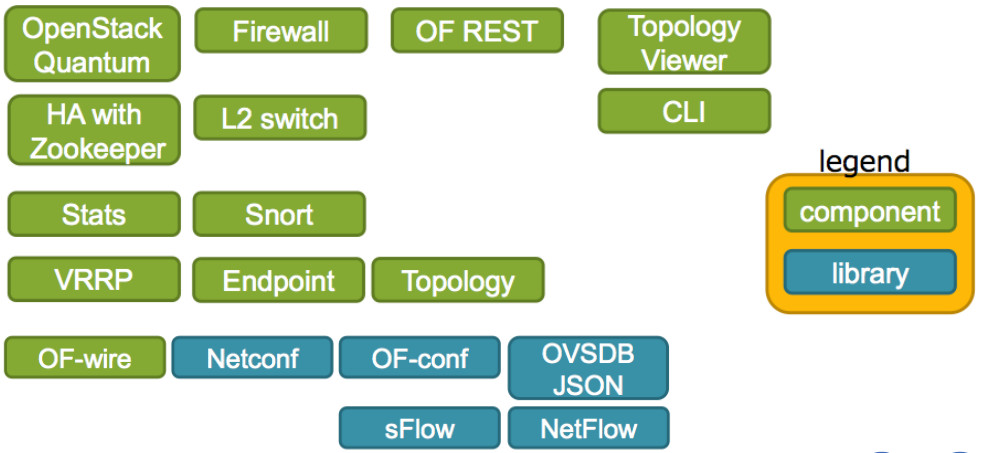
\includegraphics[width=360pt]{ryu-components.jpg}
    \caption{Principais Componentes do \textit{Ryu} \cite{ryucomponentes}.}
    \label{fig:componentes-Ryu}
    \end{center}
\end{figure}

Os principais componentes que acompanham o \textit{framework Ryu} são apresentados na figura~\ref{fig:componentes-Ryu}. Observe que o arcabouço padrão do \textit{Ryu} oferece suporte para inúmeros protocolos existentes, tais como \textit{netconf}, vrrp, xFlow, snmp e ovsdb. Além desses componentes, \textit{Ryu} possui em sua biblioteca, algumas aplicações úteis tais como um \textit{firewall} e um visualizador de topologia.



%\par \textit{Ryu} possui a desvantagem de não suportar \textit{multi-threading}, mas essa é uma das poucas desvantagens desse controlador. Em \cite{ryu_shalimov2013} pode-se encontrar uma análise desse, e de outros controladores para SDN. Dado as características desse trabalho, a falta de suporte a \textit{multi-threading} não irá afetar o desenvolvimento da pesquisa.


O controlador \textit{Ryu} é uma escolha sensata para iniciantes em  desenvolvimento de aplicações SDN, dado o grande números de componentes pré-definidos em sua arquitetura. A facilidade de se trabalhar com a linguagem Python e o vasto suporte da comunidade dessa linguagem também são os grandes atrativos desse arcabouço. Outro fator que colaborou para a escolha desse controlador é que o ambiente previsto para validação soluções de mobilidade em SDN neste TCC será o emulador de redes Netkit. A versão experimental deste emulador disponibiliza máquinas virtuais Linux com suporte ao controlador \textit{Ryu} e Openflow. Por outro lado, uma das poucas desvantagens de \textit{Ryu} é a de não suportar programação \textit{multi-threading}. \citeonline{ryu_shalimov2013} fazem uma análise detalhada desse e de outros controladores para SDN. Dados os cenários de comunicação móvel a serem investigados neste TCC, espera-se que a ausência de suporte a \textit{multi-threading} não afete o desenvolvimento do  trabalho.


\subsection{Emulador NetKit}

%@FS: remover os próximos 2 parágrafos?

%\par Um desafio comumente encontrado quando se trabalha com pesquisas em Redes de Computadores é encontrar um ambiente propício para experimentações das tecnologias desenvolvidas ou estudadas. Na Internet não é possível separar os fluxos de dados que já estão presentes na Internet de fluxos de dados em desenvolvimento, não há espaço para inovação, conforme já mencionado nos tópicos anteriores. Desse modo, quando se deseja experimentar novas tecnologias no campo das Redes de Computadores é necessário que se construa um ambiente de testes isolado, o que pode se tornar demasiadamente custoso devido ao número de elementos presentes em uma rede de computadores, tais como roteadores, servidores, entre outros. No entanto, dependendo do alvo dos estudos, é possível utilizar simuladores, ou emuladores, para realizar as experimentações necessárias. Dado as características dos estudos desse trabalho, a utilização de um emulador atenderá grande parte dos objetivos desejados. Nesse trabalho será utilizado o emulador Netkit \cite{Pizzonia} para verificação e validação das solução estudadas ou, possivelmente, desenvolvidas.

Um desafio frequentemente em pesquisas em Redes de Computadores é encontrar um ambiente propício para experimentações de novas tecnologias desenvolvidas ou estudadas. Sem o suporte de infraestrutura SDN/Openflow não é possível separar os fluxos de dados que já estão presentes na Internet dos fluxos de dados de protocolos em desenvolvimento, não havendo espaço para inovação como  discutido anteriormente. Desse modo, quando se deseja experimentar novas tecnologias em Redes de Computadores é necessário que se construa um ambiente de testes isolado, o que pode se tornar demasiadamente custoso devido ao número de elementos necessário em uma rede real, como roteadores, comutadores, servidores, enlaces de comunicação com e sem fio, entre outros. No entanto, dependendo do objeto de estudo, é possível utilizar simuladores ou emuladores para realizar os experimentações necessárias para validação de novas soluções propostas. Dadas os objetivos deste TCC, a utilização de um emulador atenderá os requisitos de validação previstos. Assim, neste trabalho será utilizado o emulador Netkit~\cite{Pizzonia} para verificação e validação das solução estudadas e desenvolvidas.

%\par O emulador Netkit oferece um ambiente leve e barato onde é possível reproduzir com fidelidade, precisão e detalhes o funcionamento de diversas tecnologias utilizadas nos inúmeros tipos de dispositivos de uma rede de computadores real. Através dessa ferramenta será possível utilizar exatamente as mesmas tecnologias que são usadas em uma rede real com a vantagem, em certo aspecto, de não possuir ruídos nem interferências de elementos internos e externos a rede, tais como congestionamentos de fluxos de dados independentes, campos eletromagnéticos, distancia física, tecnologia do material dos enlaces de transmissão, etc.

O emulador Netkit oferece um ambiente leve e de baixo custo, onde é possível reproduzir com fidelidade, precisão e detalhes o funcionamento de diversas tecnologias utilizadas em dispositivos de uma rede real. Através dessa ferramenta é possível utilizar exatamente as mesmas tecnologias que são usadas em uma rede real com a vantagem, em certo aspecto, de não possuir ruídos nem interferências (que não sejam geradas intencionalmente) de elementos internos e externos à rede, tais como: congestionamentos de fluxos de dados independentes, campos eletromagnéticos, distância física, tecnologia do material dos enlaces de transmissão, etc.


%\par O emulador Netkit é um sistema de emulação de redes baseadas em sistemas Linux que explora o User-Mode Linux (UML) \cite{umldike2001}, uma ferramenta \textit{Open Source} presente no núcleo oficial Linux que recria um sistema Linux completo (que será chamado 'máquina virtual, ou simplesmente 'VM' [\textit{Virtual Machine}]) através de uma imagem de sistema previamente armazenada na máquina hospedeira (denominado 'sistema nativo', ou simplesmente '\textit{host}'). Cada máquina virtual criada pelo UML é um processo executando sobre o sistema nativo e todos os dispositivos físicos da máquina virtual são virtualizados através de recursos do sistema nativo. Assim, discos na máquina virtual são arquivos no sistema nativo e interfaces de redes são processos em segundo plano executando no sistema nativo.

Para emular uma rede, Netkit utiliza virtualização em \textit{User-Mode Linux} (UML)~\cite{umldike2001}, que é uma forma de executar um sistema Linux completo como processos. Uma imagem de um sistema de arquivo Linux previamente armazenada na máquina hospedeira (denominado 'sistema nativo', ou simplesmente '\textit{host}') é carregada em uma máquina virtual em UML. Cada máquina virtual UML é um processo sendo executado sobre o sistema nativo e todos os recursos (CPU, RAM, HD) da máquina virtual são virtualizados a partir dos recursos físicos do sistema nativo. Assim, discos na máquina virtual são arquivos e interfaces de redes são processos em segundo plano executados no sistema nativo.


%\par Ao lançar mão sobre o UML, o Netkit pode criar quantas máquinas virtuais o hardware do sistema nativo suportar. Resta então ao Netkit a tarefa de oferecer ao usuário interfaces para que o usuário possa interagir nessas VMs e fazer com que essas VMs possam ser conectadas umas as outras como em uma rede de computadores real. Cada VM criada é apresentada ao usuário em uma janela de linha de comando comum no sistema nativo, ao executar comandos nesses terminais, esses comando estarão sendo executados somente na VM correspondente a esse terminal. A principal tarefa do Netkit é esconder do usuário as configurações necessárias para emular uma rede contendo essas máquinas virtuais. O que o usuário precisa fazer é somente dizer ao Netkit, através de arquivos textos simples, como essas máquinas estão conectadas, isto é, através de uma sintaxe simples e própria do Netkit, o usuário configura as interfaces das VMs indicando quais interfaces de rede estão no mesmo domínio. A partir desse ponto, essa rede virtual emulada (que será referenciada apenas por \textit{lab}, como na documentação oficial do \textit{software} Netkit) necessita que cada VM seja configurada apropriadamente, do mesmo modo que seriam se fossem máquinas reais conectadas em um rede física. Como em cada VM se tem um sistema Linux completo, é possível fazer uso de inúmeras tecnologias de redes \textit{Open Source} tais como Quagga, iptables, OpenFlow, tcpdump, entre inúmeras outras que podem ser instaladas em um sistema Linux real e que também são suportadas pela virtualização do Netkit. É claro que somente \textit{softwares} de linha de comando podem ser executados nessas VMs.


Ao lançar mão sobre o UML, o Netkit pode criar quantas máquinas virtuais o hardware do sistema nativo suportar. Cabe então ao Netkit a tarefa de oferecer ao usuário interfaces para que o mesmo possa interagir com as VMs, conectando umas as outras como em uma rede real. Cada VM criada é apresentada ao usuário em um terminal de comandos comum no sistema nativo. Os comandos executados nesses terminais são executados somente nas VM correspondentes a esses terminais. A principal tarefa do Netkit é mascarar internamente nas máquinas virtuais as configurações necessárias para emular uma rede, tornando-a transparente para os usuários. O que o usuário precisa fazer é configurar, através de arquivos textos simples, a forma como as VMs serão conectadas, ou seja, definir a topologia da rede desejada. Isso é feito através de uma sintaxe simples e própria do Netkit, permitindo a usuário determinar as interfaces das VMs, indicando quais delas estão ligadas no mesmo domínio de colisão. A partir desse ponto, a rede virtual emulada (que será referenciada apenas por \textit{lab}, como na documentação oficial do Netkit) necessita que cada VM seja configurada do mesmo modo que seriam se fossem máquinas reais conectadas em um rede física. Como em cada VM se tem um sistema Linux completo, é possível fazer uso das diversas ferramentas de código aberto para suporte de redes, tais como: Quagga, IPTables, Openflow, tcpdump, ou qualquer outra que possa ser instalada no sistema de arquivos das VMs. Uma limitação é que somente aplicações e ferramentas de linha de comando podem ser executados nas VMs, o que é suficiente para executar qualquer experimento que envolva transmissão de dados em redes. Além das características da virtualização de uma rede baseada em UML, o emulador Netkit apresenta facilidades que o torna especialmente útil para ensino no campo das Redes de Computadores. Esse é uma dos grandes motivações para o desenvolvimento dessa ferramenta, segundo os próprios desenvolvedores~\cite{Pizzonia}.

%\par Além dessas características que facilitam a virtualização de uma rede, a ferramenta Netkit apresenta facilidades que a torna especialmente útil para ensino no campo das Redes de Computadores, esse é um dos grandes motivos pra o desenvolvimento dessa ferramenta, segundo os próprios desenvolvedores \cite{Pizzonia}. Um \textit{lab} do Netkit, consiste apenas de arquivos textos que dizem ao Netkit quantas e como estão conectadas as máquinas virtuais desejadas, de forma que esse \textit{lab} possui poucos \textit{kilobytes} de tamanho, podendo ser facilmente transportado para outras máquinas, enviadas por e-mail, ou qualquer outra ferramente de transmissão de dados. Cada VM de um \textit{lab}, após sua inicialização, possui acesso aos arquivos do sistema nativo, de forma que é possível copiar arquivos para dentro das VMs e vice-versa. Isso tudo, aliado ao fato de que cada VM ocupa algumas dezenas de megabytes na memória da máquina hospedeira, torna o Netkit apropriado para ensino pois os estudantes podem executar os \textit{labs} em suas próprias máquinas, carregarem consigo os arquivos de configuração, além de poderem enviar facilmente esses mesmo arquivos para avaliação por parte de seus professores. Tudo o que não se refere a tecnologias de redes de computadores e que deve ser executado para as máquinas estarem logicamente conectadas é abstraído pelo Netkit de modo que cada estudante se concentra apenas naquilo que realmente interessa.

Um \textit{lab} do Netkit consiste em um arquivo texto, onde é definido quais são as VMs que compõem a rede, quais são os domínios de colisão, permitindo determinar quais interfaces das VMs serão ligadas aos domínios definidos. Um arquivo  \textit{lab.conf} possui poucos bytes de tamanho, podendo ser facilmente transportado para outras máquinas, enviadas por e-mail, copias em pendrives ou qualquer outra forma de envio. Cada VM definida em um \textit{lab.conf}, após sua inicialização, possui acesso aos arquivos do sistema nativo, de forma que é possível copiar arquivos para dentro das VMs e vice-versa. Isso tudo, aliado ao fato que cada VM ocupa algumas dezenas de megabytes na memória da máquina hospedeira, torna o Netkit apropriado para ensino. Nesse caso, estudantes podem executar os \textit{labs} em suas próprias máquinas, carregarem consigo os arquivos de configuração, além de poderem enviar facilmente esses mesmo arquivos para avaliação por parte de seus instrutores. Tudo o que não se refere a tecnologias de redes de computadores é abstraído, de modo que o estudante possa se concentrar apenas em questões técnicas e operacionais sejam pertinente à comunicação entre as VMs.

%\par Neste trabalho irá ser emulada uma rede com 7 elementos: 4 roteadores, um servidor de arquivos, um controlador \textit{Ryu} (que será descrito na seção seguinte) e a última VM simulará um dispositivo que irá se mover logicamente entre as sub-redes de cada roteador. Para simular a movimentação entre redes, será utilizado \textit{shell script} na VM que simulará o dispositivo móvel para desconectar e conectar essa VM nas diferentes sub-redes a qual estará conectada. Para cumprimento dos objetivos desse trabalho, em algumas da VMs será necessário a instalação de alguns pacotes adicionais, como o próprio controlador  \textit{Ryu}  uma implementação do padrão OpenFlow (será descrito na seção seguinte) chamada \textit{Open vSwitch} e eventuais dependências que podem surgir. Tais pacotes são disponibilizados em um versão experimental do Netkit, porém, por experiência do autor desse trabalho, esses pacotes só puderam ser corretamente utilizados após instalação diretamente de uma VM do Netkit. Ainda nisso pode-se notar a facilidade que a emulação de um sistema Linux completo oferece para seus usuários.


Neste TCC, pretende-se reproduzir um cenários de comunicação móvel através do Netkit. A rede a ser emulada será composta de poucos elementos, com até meia dezena de roteadores, um servidor de arquivos, um controlador \textit{Ryu} (que será descrito na seção seguinte) e uma última VM que representará um dispositivo móvel. Essa VM emulará um nó que irá se mover logicamente entre redes IP distintas que estarão vinculadas a cada roteador. Para representar a movimentação entre redes, será utilizado \textit{shell script} na VM que, através de comandos de terminal, simulará \textit{handovers} -- trocas de redes acesso quando o dispositivo móvel se desconecta à rede antiga se conectar à nova rede visitadas, conforme as diferentes redes IP da topologia a ser emulada. Para tanto, em algumas VMs será necessário a instalação de pacotes de softwares adicionais, como o próprio controlador  \textit{Ryu},  uma implementação do protocolo Openflow chamada \textit{Open vSwitch}, e eventuais dependências que podem surgir. Tais pacotes são disponibilizados em um versão experimental do Netkit. Porém, por experiência do autor deste trabalho, esses pacotes só puderam ser corretamente utilizados após instalação diretamente de uma VM do Netkit. Ainda com esse 
pode-se notar a facilidade que a emulação de um sistema Linux completo oferece para seus usuários.


\subsection{\textit{Shell Script}}

%\par É comum para usuários de sistemas Linux a utilização de interpretadores de comandos, tais como o \textit{bash}, sh, csh, ksh entre outros. Esses interpretadores de comandos fazem uso do \textit{Shell} do sistema operacional para executarem tarefas. O \textit{Shell} é uma camada de software responsável por fazer a interface entre o usuário e o núcleo (\textit{kernel}) do sistema. Dessa forma, é possível controlar as configurações do sistema operacional através de comandos conhecidos e bem definidos. Através do interpretador de comando, o \textit{Shell} recebe, interpreta e executa os comandos vindo do usuário. Muitas vezes os interpretadores de comandos são referenciados apenas como \textit{Shell}.


Para usuários de sistemas Linux é comum a utilização de interpretadores de comandos, tais como o \textit{bash}, \textit{sh}, \textit{csh}, \textit{ksh}, entre outros. Esses interpretadores de comandos fazem uso do \textit{Shell} do sistema operacional para executarem tarefas. O \textit{Shell} é uma camada de software responsável por fazer a interface entre o usuário e o núcleo (\textit{kernel}) do sistema \cite{shell_script-taylor}. Dessa forma, é possível controlar as configurações do sistema operacional através de comandos conhecidos e bem definidos. Através do interpretador de comando, o \textit{Shell} recebe, interpreta e executa os comandos vindo do usuário. Muitas vezes os interpretadores são referenciados apenas como \textit{Shell}. \cite{jargas2008shell}

%\par Nos interpretadores de comandos pode-se digitar comandos de forma isolada, i.e, um após o outro, ou combiná-los em uma mesma linha. É possível também colocar esses comandos em linhas subsequentes de um arquivo texto comum e invocar o \textit{Shell} sobre esse arquivo. Esse arquivo texto é então chamado um \textit{Shell Script}. \textit{Scripts} para o \textit{Shell} são amplamente utilizados em sistemas Linux para automatização das mais diversas tarefas. É uma ferramenta poderosa utilizada por administradores de sistemas e de redes facilitando e agilizando tarefas rotineiras.

Nos interpretadores de comandos pode-se inserir comandos de forma isolada ou combinar comandos, encadeando saída de um como entrada padrão de outro. É possível ainda colocar os comandos em linhas subsequentes de um arquivo texto comum e invocar o \textit{Shell} sobre esse arquivo. Esse arquivo texto é então chamado de \textit{Shell Script}. \textit{Scripts} são amplamente utilizados em sistemas Linux para automatização das mais diversas tarefas. É uma ferramenta poderosa utilizada por administradores de sistemas e de redes, facilitando e agilizando tarefas rotineiras.

%\par Nesse trabalho se fará uso dessa ferramenta para automatizar configurações das interfaces de redes das máquinas virtuais do Netkit. Através de \textit{scripts} na linguagem do \textit{Shell} do Linux será simulado a troca de rede por parte de uma máquina virtual. Essa máquina estará simulando um usuário que migra de uma rede para outra enquanto faz uso de serviços na Internet. Aqui, esse serviço será o download de um arquivo hospedado em um servidor remoto. Para a simulação de troca de rede serão utilizados comandos que ativam e desativam diferentes interfaces de redes, e entre eles, comandos de temporização. Como diferentes interfaces de redes possuem diferentes endereços, esse procedimento simulará, sem perda de generalidade, o comportamento de uma usuário que migra de uma rede para outro em um ambiente real.


Neste TCC está previsto os uso \textit{Shell Scripts} para automatizar configurações das interfaces de redes das máquinas virtuais do Netkit. Através deles será também simulado \textit{handovers}, com trocas de rede IP por parte de uma máquina virtual. Essa máquina estará simulando um usuário que migra de uma rede para outra, enquanto faz uso de serviços disponibilizados na Internet. Aqui, esse serviço será o download de um arquivo armazenado em um servidor localizado em uma rede remoto. Para a simulação de trocas de rede serão utilizados comandos que ativam e desativam diferentes interfaces de redes e, entre eles, comandos de temporização. Como diferentes interfaces de redes possuem diferentes endereços, esse procedimento simulará, sem perda de generalidade quanto aos impactos da mobilidade nas aplicações, o comportamento de um usuário que migra de uma rede IP para outra, conforme em um ambiente real.


\section{Trabalhos Relacionados}
%Soluções SDN para Mobilidade IP
%%%%%%%%%%%%%%%%%%%%%%%%%%%%%%%%%%%%%%%%%%%%%%%%%%%%%%%%%%%%%%%%%%%%%%%%%%%%%%%%%%%%%%%%%%%%%%%%%%%%%%%%%%%%%%%%%%%%%%%
\begin{comment}
    \cite{bronzino2013}, \cite{raychaudhuri2012}, \cite{cleary2009}, \cite{wang2014}, \cite{aliahmad2013}, \cite{nunes2014} e \cite{lu2016sdn}, \cite{McKeown}. \cite{nunes2014}, \cite{xu2014}, \cite{aliahmad2013}.
\end{comment}
%%%%%%%%%%%%%%%%%%%%%%%%%%%%%%%%%%%%%%%%%%%%%%%%%%%%%%%%%%%%%%%%%%%%%%%%%%%%%%%%%%%%%%%%%%%%%%%%%%%%%%%%%%%%%%%%%%%%%%%

Em~\cite{McKeown} é discutido como a Internet está inflexível para inovações e é proposto o protocolo Openflow para permitir que novas tecnologias sejam inseridas na rede. No entanto, nenhuma solução, de fato, para algum problema especifico da arquitetura atual da Internet, é descrita tecnicamente no trabalho. 

%A dissertação de mestrado do autor Edson Adriano Maravalho Avelar \cite{avelar2013} apresenta uma proposta para gerenciamento de mobilidade   utilizando Redes Definidas por Software. É uma proposta inspirada nos protocolos NetLMM e PMIPv6 \cite{RFC5213}. A proposta tem o objetivo de livrar os dispositivos móveis da responsabilidade de gerenciar sua própria mobilidade uma vez que essa função é delegada à rede através do paradigma SDN. O trabalho de \cite{avelar2013} oferece uma nova solução para tratar mobilidade a qual é avaliada em um cenario muito próximo de um cenário real. 

A dissertação de mestrado de~\citeonline{avelar2013} apresenta uma proposta para gerenciamento de mobilidade utilizando Redes Definidas por Software. É uma proposta inspirada nos protocolos NetLMM e PMIPv6~\cite{RFC5213}. A proposta tem o objetivo de livrar os dispositivos móveis da responsabilidade de gerenciar sua própria mobilidade, uma vez que essa função é delegada à rede através do paradigma SDN. A solução proposta é avaliada em um cenário muito próximo de um cenário real.

Este TCC visa construir um ambiente de emulação onde se possa realizar a implementação e avaliação de soluções para mobilidade utilizando SDN. Nesse sentido,~\citeonline{avelar2013} difere deste trabalho, pois suas propostas são implementadas e avaliadas utilizando uma combinação de dispositivos físicos e máquinas virtualizadas. Suas soluções de mobilidade foram implementadas em sistemas virtualizados, enquanto uma máquina real, executando uma aplicação, movia-se no espaço para ocorrer a troca de rede. Tal ambiente de teste é custoso. A construção de um ambiente de emulação onde se possa trabalhar com SDN visa, além de facilitar o ensino prático desse paradigma, oferecer um meio barato e rápido para avaliação de soluções desse paradigma. Outro aspecto é que em~\cite{avelar2013} utilizou-se o controlador NOX, enquanto neste TCC pretende-se utilizar um controlador contemporâneo e popular, que é o controlador~\textit{Ryu}.

%Em \cite{almeida2016} é apresentado uma nova proposta de gerenciamento de mobilidade. Essa proposta é baseada no uso de servidores de nomes globais descentralizados e na implantação do controle de mobilidades dos nós finais nos roteadores de borda da Internet. Com isso, \cite{almeida2016} visa tirar dos sistemas finais a responsabilidade de gerenciar sua própria mobilidade sem levar esse controle para o núcleo da rede. Apenas os roteadores de borda necessitariam mudanças. Para validar sua proposta, o autor utiliza a ferramenta \textit{Mininet} e a implementação de sua solução foi realizada com o controlador \textit{Floodlight}. \cite{almeida2016} se assemelha com este trabalho no sentido de utilizar um emulador de redes e no desenvolvimento de uma solução para mobilidade utilizando \textit{Openflow}. Observa-se que sua solução é baseada em soluções que não utilizam o paradigma SDN e que o controlador utilizado é o \textit{Floodlight} enquanto que nesse trabalho de conclusão de curso será utilizado o controlador \textit{Ryu}.

Em~\cite{almeida2016} é apresentado uma nova proposta de gerenciamento de mobilidade baseada no uso de servidores de nomes globais descentralizados e na implantação do controle de mobilidade dos nós em roteadores de borda da Internet. Com isso, \citeonline{almeida2016} visa tirar dos sistemas finais a responsabilidade de gerenciar sua própria mobilidade sem levar esse controle para o núcleo da rede. Apenas os roteadores de borda necessitariam de mudanças. Para validar sua proposta, o autor utiliza o emulador \textit{Mininet} e a implementação de sua solução foi realizada com o controlador \textit{Floodlight}. Este TCC se assemelha à proposta de \citeonline{almeida2016} no sentido de utilizar um emulador de redes e no desenvolvimento de uma solução para mobilidade utilizando SDN/Openflow. Observa-se, contudo, a adoção do emulador \textit{Mininet} e que o controlador utilizado é o \textit{Floodlight}, enquanto que neste TCC se fará uso do emulador Netkit e do controlador Ryu. O emulador Netkit foi desenvolvido com o objetivo de facilitar o ensino prático no campo das redes de computadores, e a configuração das interfaces de rede em cada VM se assemelha mais com um ambiente real. O controladdor \textit{Floodlight} é baseado em Java enquanto que o controlador \textit{Ryu} é escrito em Python. O suporte à linguagem Python acompanha a maioria das distribuições Linux e possuí hoje uma comunidade mais forte do que a linguagem Java, o que justifica a adoção do Controlador \textit{Ryu} nesse trabalho.

%%%%%%%%%%%%%%%%%%%%%%%%%%%%%%%%%%%%%%%%%%%%%%%%%%%%%%%%%%%%%%%%%%%%%%%%%%%%%%%%%%%%%%%%%%%%%%%%%%%%%%%%%%%%%%%%%%%%%%%%%%%%%%%%%%%
%%%%%%%%%%%%%%%%%%%%%%%%%%%%%%%%%%%%%%%%%%%%%%%%%%%%%%%%%%%%%%%%%%%%%%%%%%%%%%%%%%%%%%%%%%%%%%%%%%%%%%%%%%%%%%%%%%%%%%%%%%%%%%%%%%%


%\chapter{Trabalho Proposto: Implementação e Avaliação de Redes Móveis Definidas por Software em Ryu/OpenFlow}
\chapter{Proposta de Implementação e Avaliação de Redes Móveis Definidas por Software em Ambiente Emulado}
\label{cap:trabalho}

% O que fazer?

Afim de atingir os objetivos traçados para esse trabalho, foi realizado o planejamento das atividades e definida a metodologia que será adotada. Este trabalho visa estudar as principais soluções de mobilidade propostas na literatura que utilizam redes definidas por software e obter um guia para ensino prático no campo das Redes Definidas por Software, para tal, a metodologia adotada se dará como segue.

\section{Metodologia}
% Como fazer? Implementar topologia de rede experimental no NetKit/openFlow, Implementar solução de mobilidade com controlador  \textit{Ryu} , Validar solução no emulador Netkt 

%\par Primeiramente será preparada uma plataforma de testes para a realização dos testes com as soluções estudadas. Tal plataforma consistirá de um ambiente de emulação de redes, sendo utilizado para esse fim, o software Netkit \cite{Pizzonia}. Será utilizada a versão do Netkit que possui suporte para OpenFlow, se trata de uma versão experimental do Netkit também disponível no site dos desenvolvedores dessa ferramenta. 

Primeiramente, será preparada uma plataforma experimental para a realização dos testes das soluções estudadas. Tal plataforma consistirá de um ambiente de emulação de redes, sendo previsto para esse fim, o emulador Netkit~\cite{Pizzonia}. Será utilizada a versão do Netkit que possui suporte para OpenFlow, a qual é uma versão experimental do Netkit disponível no site oficial do emulador. 


%\par Com o software Netkit instalado, será implementado uma topologia de rede simples onde será simulado a mobilidade de um determinado sistema final entre redes distintas. Para esse procedimento será utilizado Shell Script. Como já citado, serão implementas as soluções utilizando OpenFlow, para esse fim, será utilizado os softwares \textit{Ryu} e OpenVSwitch. O  \textit{Ryu} , como já apresentado, é um controlador Openflow, e o OpenVSwitch é a implementação de um Switch OpenFlow na linguagem C. Outras tecnologias que serão utilizadas durante o desenvolvimento dos trabalhos são: Shell Script, protocolo de roteamento RIP através do pacote Quagga, disponível nos sistemas Linux, e, obviamente, Redes IP.

Uma vez devidamente instalada a versão experimental do Netkit, será implementada uma topologia de rede simples onde será simulado a mobilidade de um determinado sistema final entre redes distintas. Para esse procedimento será utilizado \textit{Shell Script}. Como discutido anteriormente, pretende-se implementar soluções de mobilidade utilizando SDN/Openflow. Para esse fim, será utilizado o arcabouço \textit{Ryu}, com o suporte do pacote OpenVSwitch, o qual implementa o protocolo Openflow de modo a habilitar um comutador SDN. Além de \textit{Shell Script}, outras ferramentas de suporte previstas durante o desenvolvimento deste trabalho são protocolos de roteamento, como RIP e OSPF, suja implementação é fornecida pelo pacote Quagga, disponível para sistemas Linux e já instaladas no sistema de arquivo das VMs do Netkit.

%\par A topologia de rede que será implementada será baseada na figura 2. Nela, observá-se a presença de um servidor, quatro roteadores (R1, R2, R3 e R4), um controlador e um sistema final denominado Cliente.

A topologia de rede que se pretende implementar será baseada na Figura~\ref{fig:Proposta_Topologia_Experimento}. Nela observa-se a presença de um Servidor, quatro roteadores (R1, R2, R3 e R4), um controlador e um sistema final denominado Cliente.

\begin{figure}[ht]
    \begin{center}  
    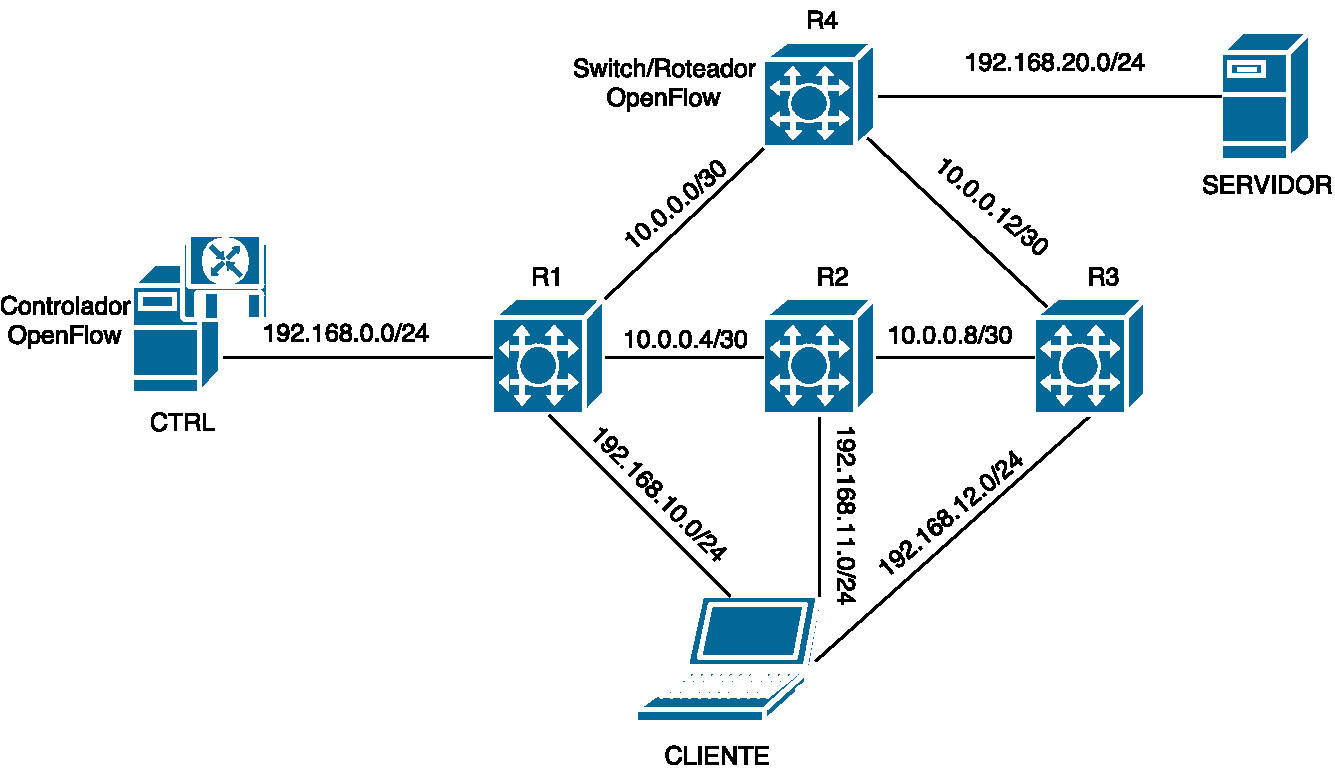
\includegraphics[width=400pt]{rede-experimento-1-27122016.pdf}
    \caption{Proposta de uma topologia de rede experimental a ser implementada.}
    \label{fig:Proposta_Topologia_Experimento}
    \end{center}
\end{figure}

%\par O servidor presente nessa topologia será de onde o cliente fará o download de um arquivo. Durante o download do arquivo, um script estará em execução no cliente emulando a mobilidade desse sistema final em relação as redes de acesso que ele possuí. Quando os roteadores interligados ao cliente detectarem mudanças em suas conexões com o cliente, eles irão entrar em contato com o controlador solicitando novas regras de encaminhamento de pacote. Esse procedimento será implementado através do OpenVswitch e do Controlador  \textit{Ryu}. Tanto a implementação de como cada \textit{switch} detectará a mudança de rede, como o modo que o Controlador decidirá que novas regras enviar para cada \textit{switch} faz parte da solução de mobilidade pesquisada e implementada.

O servidor previsto nessa topologia será a fonte de onde o cliente fará o download de um conteúdo. Durante o download do arquivo, um script estará em execução no cliente, simulando a mobilidade desse sistema final em relação as redes de acesso que ele visita. Quando os roteadores R1, R2 ou R3 receberem tráfego do cliente móvel, os mesmos irão requisitar ao controlador regras de encaminhamento esse fluxo, caso não possuam. Esse procedimento será programado com framework~\textit{Ryu} com suporte de OpenVswitch nos roteadores. Tanto a implementação de como cada os roteadores detectarão a mobilidade do cliente quanto a ação que o controlador tomará faz parte da solução de mobilidade a ser  pesquisada e implementada.


%\par Após preparada a plataforma de testes, teremos um ambiente livre de interferências onde se poderá obter dados teóricos confiáveis de QoS como vazão, atrasos, perda de pacotes, etc. As pesquisas serão realizadas através da leitura de inúmeros artigos científicos publicados nos mais diversos meios de difusão de publicações acadêmicas, mas principalmente, aqueles voltados para o universo tecnológico, como o IEEE.

Após preparada a plataforma de testes, teremos um ambiente livre de interferências onde se poderá obter dados experimentais confiáveis de QoS, como vazão, atraso, variação do atraso e perda de pacotes. A investigação será realizada através de levantamento contínuo do estado da arte através de artigos científicos disponibilizados em veículos de difusão científica, principalmente aqueles voltados para tecnologia da informação e comunicação, como o IEEE, ACM e Elsevier.

\section{Resultados Esperados}
% O que se espera ao concluir o trabalho? 
% Implementar rede experimental no netkit
% Implementar solução de mobilidade com controlador Ryu
% Avaliação de desempenho de solução de mobilidade implementada (discutir métricas: tempo de desconexão durante a mobilidade, vazão durante mobilidade, ...)

%\par Espera-se que esse trabalho realize a implementação de algumas soluções para mobilidade utilizando Redes Definidas por Software. Para tal, espera-se também que se construa um ambiente de emulação de redes que suporte esse novo paradigma. 
Espera-se realizar a implementação de soluções de mobilidade utilizando Redes Definidas por Software. Para tal, é necessário a construção de um ambiente de emulação de redes que suporte esse novo paradigma.

%\par Após a construção do ambiente de emulação e implementação das soluções, serão realizados testes e avaliação das soluções implementadas, de modo que espera-se obter parâmetros de QoS (Qualidade de Serviço). O principal parâmetro para avaliação da qualidade de serviço de uma solução para mobilidade é o tempo de desconexão, mas serão considerados também, a vazão, latência e taxa de erro.

Após a construção do ambiente de emulação e implementação das soluções, serão planejados experimentos para coleta de parâmetros de QoS e então avaliação de desempenho das soluções implementadas. O principal indicar de desempenho de solução de mobilidade é o atraso, especificamente a latência de desconexão, o qual será analisado juntamente com os outros parâmetros, de perda e vazão.

%\par Espera-se também  a confecção de um guia de instalação e configuração do ambiente de emulação construído que possa guiar futuros estudantes no campo das Redes de Computadores.

Espera-se, ainda, a confecção de um documento com informações técnicas para implantação do ambiente de emulação construído. Tal documento será útil para futuros estudantes iniciarem investigações nessa área.


\section{Cronograma}
%definir as etapas: (1-revisão bibliográfica, 2-implementação da rede experimental, 3-implementação da solução de mobilidade, 4-avaliação de desempenho
%criar com o cronograma de 9 meses

%O desenvolvimento deste trabalho se dará conforme o seguinte quadro:

O desenvolvimento deste trabalho tem seguido o cronograma de atividades da Tabela~\ref{tabela:cronograma}.


\begin{table}[!ht]
\caption{Cronograma de atividades.} 
\label{tabela:cronograma}
\begin{center}
\begin{tabular}{|c|c|c|c|c|c|c|c|c|c|c|c|c|}
\hline
{\textbf{Atividade}} & Jul & Ago & Set & Out & Nov & Dez & Jan & Fev & Mar & Abr & Mai & Jun \\
\hline
$(a_1)$              & X   & X   &  X  &     &     &     &     &     &     &     &     &\\
\hline
$(a_2)$              &     &     &  X  &  X  &  X  &     &     &     &     &     &     &\\
\hline
$(a_3)$              &     &     &     &     &  X  &     &     &     &     &     &     &\\
\hline
$(a_4)$              &     &     &     &     &     &  X  &     &     &     &     &     &\\
\hline
$(a_5)$              &     &     &     &  X  &  X  &  X  &     &     &     &     &     &\\
\hline
$(a_6)$              &     &     &     &     &     &     &  X  &  X  &     &     &     &\\
\hline
$(a_7)$              &     &     &     &     &     &     &     &  X  &  X  &     &     &\\
\hline
$(a_8)$              &     &     &     &     &     &     &     &     &  X  &     &     &\\
\hline
$(a_9)$              &     &     &     &     &     &     &     &     &  X  &  X  &     &\\
\hline
$(a_{10})$             &     &     &     &     &     &     &     &     &     &  X  &  X  &\\
\hline
$(a_{11})$             &     &     &     &     &     &     &     &     &     &     &     &  X \\
\hline
\end{tabular}
\end{center}
\end{table}


As atividades previstas são:

\begin{enumerate}[label=$(a_{\arabic*})$]
 \item  Levantamento bibliográfico sobre fundamentação teórica: Redes IP, Computação Móvel, Gerenciamento de Mobilidade, Redes Definidas por Software.
 \item  Levantamento bibliográfico sobre tecnologias envolvidas no desenvolvimento do trabalho proposto: Openflow, Emulador NetKit, \textit{Framework Ryu}, \textit{Shell Script}.
 \item  Levantamento bibliográfico sobre trabalhos relacionados.
 \item  Defesa do TCC-I
 \item  Implementação e preparação de uma plataforma de testes em ambiente emulado.
 \item  Investigação de soluções de mobilidade em SDN.
 \item  Implementação e preparação das soluções escolhidas.
 \item  Planejamento e execução de experimentos no ambiente de emulação.
 \item  Avaliação de desempenho e discussão dos resultados.
 \item  Escrita da monografia.
 \item  Defesa do TCC-II.
\end{enumerate}

Durante a atividade $(a_1)$ realizou-se uma revisão sobre os conceitos fundamentais para se entender o modo como as transmissão de dados ocorrem da Internet, de modo a obter uma profunda compreensão do problema que nós móveis sofrem ao trocar de rede.

Na atividade $(a_2)$ realizou-se a investigação e documentação das ferramentas que serão utilizadas nesse trabalho afim de estudar soluções para mobilidade utilizando o paradigma das Redes Definidas por Software.

Durante a atividade $(a_3)$ foi realizado a investigação de trabalhos existentes na literatura que discorrem sobre soluções para mobilidade na Internet utilizando SDN. Procurou-se entender as diferentes formas de trabalhar com SDN, as opções existentes e as vantagens que as ferramentas que aqui serão utilizadas sobre outras utilizadas em outros trabalhos.

Na atividade $(a_4)$ foi reservado um tempo para realizar as correções propostas pela banca de avaliação deste trabalho.

Durante a realização da atividade $(a_5)$ realiza-se a instalação da versão experimental do software Netkit. Esta versão não possui um pacote completo de instalação a exemplo de sua versão estável. Somente são disponibilizado os arquivos referentes ao sistema de arquivos e \textit{kernel} do software, de modo que sua instalação somente é realizada através da construção de um diretório funcional do software Netkit utilizando esses arquivos nos lugares corretos. Devido à essa complexidade, foi produzido um guia de instalação dessa ferramenta para documentar e facilitar futuras instalações desse software.

Na atividade $(a_6)$ realizar-se-á pesquisa na literatura em busca de diferentes soluções para mobilidade utilizando OpenFlow. Essas soluções serão estudadas e algumas delas escolhidas para implementação e avaliação nas etapas futuras.

Durante a atividade $(a_7)$ será realizada a implementação das soluções escolhidas. Além da implementação propriamente dita, essa atividade prevê o estudo da linguagem de programação \textit{Python}, que o autor do trabalho ainda não domina suficientemente.

Na atividade $(a_8)$ realizar-se-á diferentes testes das soluções implementadas. Serão captados diferentes dados durante transmissões de dados entre dois sistemas finais no ambiente emulado, sendo que durante as transmissões será emulado a mobilidade do nó 'cliente'.

Durante a atividade $(a_9)$ será realizada estudo dos resultados obtidos. A partir de métricas de QoS, os dados obtidos nos testes serão utilizados para se determinar a qualidade de cada solução, assim como a viabilidade da utilização de SDN.

A atividade $(a_{10})$ reserva-se a documentação e formatação de todo o trabalho executado.

Finalmente, na $(atividade_{11})$, realiza-se a defesa desse trabalho, assim como as correções propostas pela banca de avaliação.

\chapter{Conclusões Parciais}
\label{cap:conclusoes}
% contribuições esperadas do seu trabalho
% dificuldades encontradas até o momento

%\par Até o momento, foi realizada a construção e configuração do ambiente de emulação de rede. Foi implementado uma topologia de rede simples onde será emulado o ambiente de mobilidade no qual as soluções de mobilidade em SDN serão aplicadas. 

Até o momento, foi realizado a revisão bibliográfica e iniciou-se a construção e configuração do ambiente de emulação de rede. Foi implementado uma topologia de rede simples no ambiente de emulação, conforme ilustra a Figura~\ref{fig:Topologia_Experimento}, onde as soluções de mobilidade em SDN serão avaliadas durante o tratamento dos impactos da mobilidade da VM Cliente.

\begin{figure}[h]
    \begin{center}  
    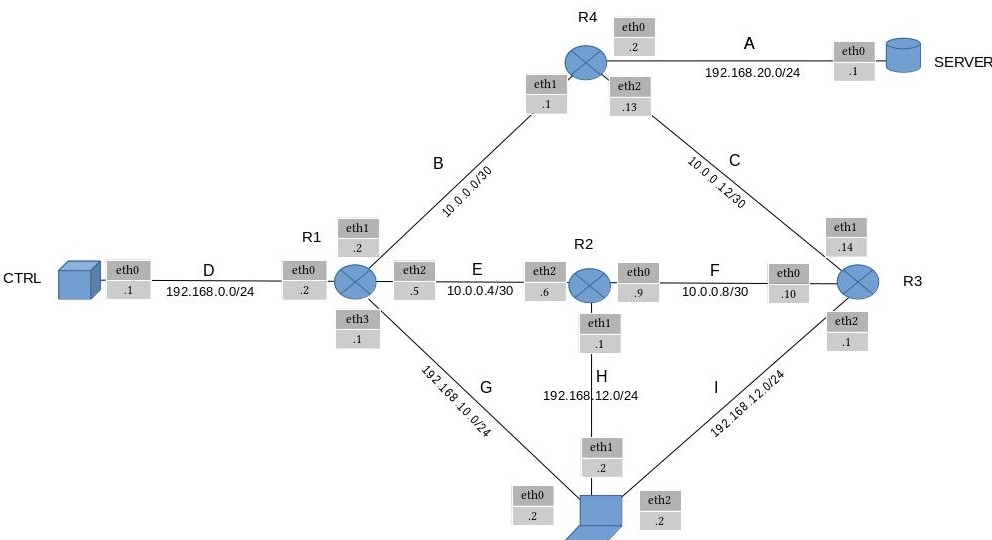
\includegraphics[width=450pt]{TOPOLOGIA-REDE-EXP1.jpg}
    \caption{Topologia de rede do Experimento.}
    \label{fig:Topologia_Experimento}
    \end{center}
\end{figure}

%\par Um \textit{script} Shell foi implementado para simular a troca de rede por parte do Cliente. Esse \textit{script} desativará e ativará as interfaces de rede do cliente de maneira alternada e subsequente de modo que apenas uma das interfaces estará ativa em qualquer momento. Esse procedimento simula o momento em que um dispositivo abandona um rede e se conecta em outra.

Na parte de desenvolvimento, no escopo da construção do ambiente de emulação, foi também iniciada a implementação de um \textit{script} Shell para simular a troca de rede por parte do Cliente. Esse \textit{script} desativará e ativará as interfaces de rede do cliente de maneira alternada e subsequente de modo que apenas uma das interfaces estará ativa em qualquer momento. Esse procedimento representará o momento em que um dispositivo abandona um rede e se conecta em outra. Como parte da construção desse ambiente de emulação, será implementado também um \textit{script} para execução dos experimentos planejados e obtenção dos indicadores de QoS resultados das transmissões do dispositivo móvel Cliente para, então, realizar a avaliação das soluções de mobilidades a serem implementadas. 



%\par Uma dificuldade encontrada foi a obtenção do correto funcionamento das ferramentas necessárias para o suporte ao paradigma SDN. O controlador \textit{Ryu} pré-instalado no emulador Netkit não funcionou corretamente, apresentando erros na fase de testes das ferramentas. Uma nova instalação teve que ser realizada, tal instalação não foi tão simples de se realizar como seria em um ambiente real. As máquinas virtuais do Netkit possuem um sistema de arquivo baseada em uma distribuição antiga do sistema Debian, existem incompatibilidades que acarretam em falhas imprevisíveis. Ainda não pode-se determinar qual a melhor forma de se instalar o controlador  \textit{Ryu}, dado que dependências de pacotes ainda não foram corretamente identificadas.

Uma dificuldade encontrada foi a obtenção de documentação para o correto funcionamento das ferramentas necessárias para o suporte ao paradigma SDN. O controlador \textit{Ryu} pré-instalado no emulador Netkit não funcionou corretamente, apresentando erros na fase de testes das ferramentas. Uma nova instalação teve de ser realizada, contudo, não foi tão simples de se realizar a instalação como seria em um ambiente real. As máquinas virtuais do Netkit possuem um sistema de arquivo baseada em uma distribuição antiga do Linux Debian. Portanto, diversas incompatibilidades acarretaram em falhas imprevisíveis. Para que fosse obtido o correto funcionamento do controlador \textit{Ryu} foi necessário remover o controlador \textit{Ryu} e todas as suas dependências, do sistema de arquivo do Netkit. Após realizada a remoção , foi realizada uma nova instalação do controlador e de suas dependências através dos pacotes de instalação disponíveis no \textit{site} oficial da ferramenta. As dependências foram instaladas conforme mensagens de erros surgiam nas tentativas de execução de uma aplicação de teste do controlador \textit{Ryu}. Para isso, foi necessário conectar uma máquina virtual do Netkit à internet.

%\par Também foi constatado mal funcionamento da ferramenta OpenVSwitch que acompanha o software Netkit. Esse software será executado nas máquinas virtuais que emularão o funcionamento de um switch Openflow na infraestrutura da Internet. Também foi realizada uma nova instalação do OpenVSwitch.

Outra ferramenta que acompanha a versão experimental do Netkit e que também apresentou mau funcionamento foi OpenVSwitch. Essa ferramenta implementa o protocolo Openflow e será executada nas máquinas virtuais responsáveis pelo roteamento na rede. Também foi realizada uma nova instalação do OpenVSwitch a exemplo da instalação do controlador \textit{Ryu}.



% ---
% Finaliza a parte no bookmark do PDF, para que se inicie o bookmark na raiz
% ---
\bookmarksetup{startatroot}% 
% ---



% ----------------------------------------------------------
% ELEMENTOS PÓS-TEXTUAIS
% ----------------------------------------------------------
\postextual


% ----------------------------------------------------------
% Referências bibliográficas
% ----------------------------------------------------------
%\bibliographystyle{plain}
\bibliography{_references}

% ----------------------------------------------------------
% Glossário
% ----------------------------------------------------------
%
% Consulte o manual da classe abntex2 para orientações sobre o glossário.
%
%\glossary

% ----------------------------------------------------------
% Apêndices
% ----------------------------------------------------------

% ---
% Inicia os apêndices
% ---
%\begin{apendicesenv}

% Imprime uma página indicando o início dos apêndices
%\partapendices

% ----------------------------------------------------------
%\chapter{Título de Apêndice}
% ----------------------------------------------------------


% ----------------------------------------------------------
%\chapter{Título do Apêndice}
% ----------------------------------------------------------


%\end{apendicesenv}
% ---


% ----------------------------------------------------------
% Anexos
% ----------------------------------------------------------

% ---
% Inicia os anexos
% ---
%\begin{anexosenv}

% Imprime uma página indicando o início dos anexos
%\partanexos

% ---
%\chapter{Título do Anexo}
% ---

%\end{anexosenv}

\end{document}